\documentclass[ %final, print %,german
  %draft,    % omit title page, listings, and particular chapters selected below using include only
	%german,   % titles for a thesis in German, A4 paper
	%print,    % the printed version does not use colored links
	final,    % removes all TODOs
]{tex/ttthesis}
\usepackage{xparse}
\usepackage{caption}
% Color Scheme http://colorschemedesigner.com/#3w40I--ALK-K-
% Base Color of the OVGU INF logo, tetraed, -45
\definecolor{blue1}{RGB}{0,105,180} % gray 95
\definecolor{blue2}{RGB}{40,87,121}
\definecolor{blue3}{RGB}{0,57,97}
\definecolor{blue4}{RGB}{76,166,230}
\definecolor{blue5}{RGB}{136,191,230}
\definecolor{orange1}{RGB}{255,144,0} % gray 133
\definecolor{orange2}{RGB}{171,121,56}
\definecolor{orange3}{RGB}{137,78,0}
\definecolor{orange4}{RGB}{255,181,84}
\definecolor{orange5}{RGB}{255,210,151}
\definecolor{green1}{RGB}{11,215,0} % gray 75
\definecolor{green2}{RGB}{52,144,48}
\definecolor{green3}{RGB}{6,116,0}
\definecolor{green4}{RGB}{88,241,80}
\definecolor{green5}{RGB}{148,241,143}
\definecolor{red1}{RGB}{253,0,6} % gray 86
\definecolor{red2}{RGB}{170,56,59}
\definecolor{red3}{RGB}{136,0,3}
\definecolor{red4}{RGB}{254,84,88}
\definecolor{red5}{RGB}{254,151,154}

\definecolor{background}{named}{white}
\definecolor{bgborder}{named}{black}
\definecolor{comment}{named}{red3}

\definecolor{blue}{named}{blue1}
\definecolor{green}{named}{green1}
\definecolor{red}{named}{red1}
\definecolor{orange}{named}{orange1}

\definecolor{pdflinkcolor}{named}{blue3}
\definecolor{pdfcitecolor}{named}{green3}

\usepackage{listings} % source code listings

%\renewcommand\lstlistingname{Quelltext}

\lstdefinestyle{java}{
%code formatting
	language=Java,
	tabsize=4,
	breaklines=false,
	basicstyle=\fontfamily{pcr}\footnotesize\selectfont,
	commentstyle=\fontshape{it}\color{darkgray}\selectfont,
	keywordstyle=\fontseries{b}\selectfont,
	stringstyle=\fontfamily{cmr}\selectfont,
%line numbering
	numbers=left,
	numberstyle=\footnotesize,
%frame properties
	captionpos=b,
	frame=single,%trblTRBL
	framesep=3pt,
	xleftmargin=4pt,
	xrightmargin=4pt,
	rulecolor=\color{bgborder},
}

\usepackage{pgfplots}
\usepackage{tikz}
	\usetikzlibrary{arrows,positioning,backgrounds,fit,trees} 
	\usetikzlibrary{fadings,shapes.geometric}
	\usetikzlibrary{decorations,scopes,calc,decorations.pathreplacing}
	\usetikzlibrary{shapes}		%tikz package to split shapes
	\usetikzlibrary{3d}
% Tortendiagramme
\newcommand{\slice}[4]{
  \pgfmathparse{0.5*#1+0.5*#2}
  \let\midangle\pgfmathresult

  % slice
  \draw[thick,
	%fill=background
	] (0,0) -- (#1:1) arc (#1:#2:1) -- cycle;

  % outer label
  \node[label=\midangle:#4] at (\midangle:1) {};

  % inner label
  \pgfmathparse{min((#2-#1-10)/110*(-0.3),0)}
  \let\temp\pgfmathresult
  \pgfmathparse{max(\temp,-0.5) + 0.8}
  \let\innerpos\pgfmathresult
  \node at (\midangle:\innerpos) {#3};
}
\newcommand{\mypiechart}[2]{
	\begin{tikzpicture}[scale=#1]
		\newcounter{a}
		\newcounter{b}
		\foreach \p/\t in {#2}
			{
				\setcounter{a}{\value{b}}
				\addtocounter{b}{\p}
				\slice{\thea/100*360}
							{\theb/100*360}
							{\p\%}{\t}
			}
	\end{tikzpicture}
}


% surrounding TODOs with this command, gives you the ability to remove all if necessary
\iffinal{
	\newcommand{\todo}[1]{}
	\newcommand{\todots}{}
}{
	\newcommand{\todo}[1]{{\color{comment}\textit{[#1]}}}
	\newcommand{\todots}{\todo{\ldots}}
}

% propositional formulas
\newcommand{\pand}{\wedge}
\newcommand{\por}{\vee}
\newcommand{\pnot}{\neg}
\newcommand{\pequals}{\Leftrightarrow}
\newcommand{\pimplies}{\Rightarrow}
\newcommand{\pnimplies}{\nRightarrow}
\newcommand{\patmostone}{\mbox{\textit{atmost1}}}
\newcommand{\pchooseone}{\mbox{\textit{choose1}}}

% mathematical definitions and theorems
\newtheorem{definition}{Definition}[chapter]
\newtheorem{theorem}{Theorem}[chapter]
\newtheorem{lemma}{Lemma}[chapter]

% print URLs not in Typewriter Font
\def\UrlFont{\rm}

% empty page without page number, continue on the next right page
\newcommand{\blankpage}{\clearpage{\pagestyle{empty}\cleardoublepage}}

% index stuff
\makeatletter
\def\mydotfill{\leavevmode\xleaders\hb@xt@ .44em{\hss.\hss}\hfill\kern\z@}
\makeatother
\def\bold#1{{\bfseries #1}}
\newbox\dbox \setbox\dbox=\hbox to .4em{\hss.\hss} % dot box for leaders
\newskip\rrskipb \rrskipb=.5em plus3em % ragged right space before break
\newskip\rrskipa \rrskipa=-.17em plus -3em minus.11em % ditto, after
\newskip\rlskipa \rlskipa=0pt plus3em % ragged left space after break
\newskip\rlskipb \rlskipb=.33em plus-3em minus.11em % ragged left before break
\newskip\lskip \lskip=3.3\wd\dbox plus1fil minus.3\wd\dbox % for leaders
\newskip \lskipa \lskipa=-2.67em plus -3em minus.11em %after leaders
\mathchardef\rlpen=1000 \mathchardef\leadpen=600
\def\rrspace{\nobreak\hskip\rrskipb\penalty0\hskip\rrskipa}
\def\rlspace{\penalty\rlpen\hskip\rlskipb\vadjust{}\nobreak\hskip\rlskipa}
\let\indexbreak\rlspace
\def\raggedurl{\penalty10000 \hskip.5em plus15em \penalty0 \hskip-.17em plus-15em minus.11em}
\def\raggeditems{\nobreak\hskip\rrskipb \penalty\leadpen \hskip\rrskipa %
\vadjust{}\nobreak\leaders\copy\dbox\hskip\lskip %
\kern3em \penalty\leadpen \hskip\lskipa %
\vadjust{}\nobreak\hskip\rlskipa}
\renewcommand*\see[2]{\rlspace\emph{\seename}~#1} % from makeidx.sty

\ifgerman{\renewcommand{\lstlistingname}{Quelltext}}{\renewcommand{\lstlistingname}{Source code}}

%*********************************************************************%http://www.coppeliarobotics.com/downloads.html
% META                                                                %
%*********************************************************************%
\ifgerman{
  \newcommand{\university}{Otto-von-Guericke-Universität Magdeburg}
  \newcommand{\school}{Fakultät für Informatik}
}{
  \newcommand{\university}{University of Magdeburg}
  \newcommand{\school}{School of Computer Science}
}
\newcommand{\logo}{
\includegraphics[trim=0mm 0mm 50mm 0mm,clip,height=3cm]{INF_SIGN_druck}}


\newcommand{\advisorone}{Prof. {Sanaz Mostaghim}}
\newcommand{\departmentone}{\ifgerman{Institut für Intelligente Systeme}{Department of Intelligent Systems} }

\newcommand{\advisortwo}{Christoph Steup}
\newcommand{\departmenttwo}{\ifgerman{Institut für Intelligente Systeme}{Department of Intelligent Systems} }

% Thesis kind
%\ifgerman{\newcommand{\thesiskind}{Masterarbeit}}{\newcommand{\thesiskind}{Master's Thesis}}
\ifgerman{\newcommand{\thesiskind}{Projektbericht}}{\newcommand{\thesiskind}{Digital Engineering Project}}
%\newcommand{\thesiskind}{Diplomarbeit} %do not translate
%\ifgerman{\newcommand{\thesiskind}{Doktorarbeit}}{\newcommand{\thesiskind}{Dissertation}}

\ifgerman{

}{
	\newcommand{\theforename}{Lukas}
	\newcommand{\thesurname}{Mäurer}
	\newcommand{\thesecondforename}{Vladimir}
	\newcommand{\thesecondsurname}{Velinov}
	\newcommand{\thetitle}{Mixed-reality Simulation of Quadcopter-Swarms}
	\newcommand{\thedate}{March 17}
}
\newcommand{\theyear}{2016}

%*********************************************************************%
% SETUP                                                               %
%*********************************************************************%

% meta informations of the document
\hypersetup{
 pdfauthor={\theforename\ \thesurname},
 pdftitle={\thetitle}
}



% open index file
\ifnotdraft{\makeindex}

%*********************************************************************%
% THE DOCUMENT                                                        %
%*********************************************************************%

\makeglossaries
\begin{document}

%*********************************************************************%
% ACRONYMS                                                            %
%*********************************************************************%

% HOWTO: \gls{IDE} for singular or \glspl{IDE} for plural with 's
\newacronym{IMU}{IMU}{Inertial Measurement Unit}
\newacronym{AHRS}{AHRS}{Attitude Heading Reference System}
\newacronym{UAV}{UAV}{Unmanned Air Vehicle}
\newacronym{PID}{PID}{Proportional-Integral-Derivative}
\newacronym{GUI}{GUI}{Graphical User Interface}

%\newacronym{}{}{}
%\glsaddall % use only if you have acronyms that occur only in graphics

% set the path where graphics are located
\graphicspath{{pics/}}

\ifnotdraft{
	\frontmatter
	\pagenumbering{roman}
	\newcommand{\theauthor}{\theforename\ \thesurname}
\newcommand{\theauthorr}{\thesurname,\ \theforename}
\newcommand{\thesecondauthor}{\thesecondforename\ \thesecondsurname}
\begin{titlepage}
 \thispagestyle{empty}
 \begin{center}
  {\university}\\[0.4cm]
  {\school}\\[2.0cm]
  \begin{figure}[h]
   \hbox{}\hfill
    \begin{minipage}[t]{\textwidth}
      \begin{center}
        \logo
      \end{center}
    \end{minipage} 
   \hfill\hbox{}
  \end{figure}\ \\[0.4cm]
  {\large \thesiskind \\[1.6cm]}
  {\huge\bf \thetitle \\[1.6cm]}
  { \ifgerman{Autor:}{Author:}}\\[0.4cm]
  {\huge \theauthor}\\[0.2cm]
  {\huge \thesecondauthor}\\[0.2cm]
  {\large\thedate, \theyear}\\[0.8cm]
  {\ifgerman{Betreuer:}{Advisors:}}\\[0.4cm] 
  {\large
\advisorone
  }\\[0.2cm]
  {
\departmentone
  }\\[0.8cm]
  {\large
\advisortwo\ 
  }\\[0.2cm]
  {
\departmenttwo\ 
  }
 \end{center}
\end{titlepage}

%%%%%%%%%%%%%%%%%%%%%%%%%%%%%%%%%%%%%%%%%%%%%%%%%%%%%%%%%%%%%%%%%%%%%%%%%%%%
%%% Titelrückseite: Bibliographische Angaben
%%%%%%%%%%%%%%%%%%%%%%%%%%%%%%%%%%%%%%%%%%%%%%%%%%%%%%%%%%%%%%%%%%%%%%%%%%%%

\thispagestyle{empty}
\vspace*{\fill}
\begin{minipage}{15.0cm}
\textbf{\theauthorr:}\\
\emph{\thetitle\\}
\thesiskind, \university, \theyear.
\end{minipage}
\newpage

%Sperrvermerk
\ifnotdraft{
	\cleardoublepage
	\phantomsection
	\printindex
	\include{tex/sperrvermerk}
}

	\include{chapters/danksagung}
	\blankpage

	%\chapter*{Acknowledgements}
	%\ldots
	%\blankpage
}



%*********************************************************************%
% LISTINGS                                                            %
%*********************************************************************%

\ifnotdraft{
	{\parskip 0pt\tableofcontents} % toc bitte einzeilig
	\blankpage

	\ifgerman{
		%\listoffigures
		%\addcontentsline{toc}{chapter}{Abbildungsverzeichnis}

		%\listoftables
		%\addcontentsline{toc}{chapter}{Tabellenverzeichnis}

		%\renewcommand{\lstlistlistingname}{Quelltextverzeichnis}
		%\lstlistoflistings
		%\addcontentsline{toc}{chapter}{Quelltextverzeichnis}

		\renewcommand*{\firstacronymfont}[1]{\emph{#1}}
		\printglossary[type=acronym,title=Abkürzungsverzeichnis,toctitle=Abkürzungsverzeichnis]
	}{
		\listoffigures
		\addcontentsline{toc}{chapter}{List of Figures}

		\listoftables
		\addcontentsline{toc}{chapter}{List of Tables}

		\renewcommand{\lstlistlistingname}{List of Code Listings}
		\lstlistoflistings
		\addcontentsline{toc}{chapter}{List of Code Listings}

		\renewcommand*{\firstacronymfont}[1]{\emph{#1}}
		\printglossary[type=acronym,title=List of Acronyms,toctitle=List of Acronyms]
	}
}

%*********************************************************************%
% CHAPTERS                                                            %
%*********************************************************************%

\mainmatter
\pagenumbering{arabic}

\ifgerman{\chapter{Einleitung}}{\chapter{Introduction}}
%- Hintergrund
%- Motivation
%- Ziele
%- Aufgaben
%- Allgemeine Beschreibung des Projektes
%- Worum geht es in dieser Arbeit?
%- Wer hat die Arbeit veranlasst und wozu?
%- Wer soll von den Ergebnissen profitieren?
%- Welches Problem soll gelöst werden? Warum?
%- Unter welchen Umständen braucht man eine Verbesserung?
%- Was ist der Stand der Technik?
%- Welche noch offenen Probleme gibt es?
%- Worin unterscheidet sich mein Ansatz von den bisherigen?
%- Welche Ziele hat die Arbeit?
%- Wie will ich diese Ziele erreichen?
%- Was habe ich im Einzelnen vor?


\section{Motivation}

The work presented in this document was carried out at the Swarm Lab at the Otto-von-Guericke-University Magdeburg. The research focus of the working group lies on implementing and investing swarm algorithms in practice by using small indoor quadcopter. The used FINken quadcopter were developed in association with the working group and are small, but powerfull and are highly extensible. As the research focus on swarm intelligence puts an interest on autonomous behaviour, the copter fly without any external reference and rely solely on onboard sensors.

As the copter were developed in the working group and were designed with a focus on modularity, they are under constant change. Testing new changes of the copter, e.g. new control or behavioural algorithms alway poses a certain risk to the hardware due to crashs caused by bugs. Thus, a simulation tool for the quadcopters to test new software is desirable to be able to do a safe first evaluation of newly implemented ideas. A less abstract solution than a pure simulation could be a mixed reality simulation, where the behaviour of real and simulated quadcopter could be directly compared.

\todo{who needs the results}

\todo{what are the problems to be solved?}

\todo{what are existing solutions, what's different in this approach, what is the improvement}


       


  
\section{Problem Statement}
    
    \todo{what are the goals}
    \todo{how are we going to reach this goals}
    \todo{what is to be done}
 
         
\section{Outline}
    
  \todo{short description of the sections}
   % use " in \ref{} to reference "\labels{}" in the document
   
%\ifgerman{\chapter{Grundlagen}}{\chapter{Background}}
\label{sec:background}
%- Allgemeine Wissensgrundlagen des Fachgebiets
%- Spezielle Grundlagen, die für das Verständnis erforderlich sind
%- Rahmenbedingungen für die Arbeit
%- Ausführungen zum Stand des Wissens / der Technik
%Als Leitprinzip gilt: Nur Informationen erwähnen, die
%- später benötigt werden,
%- notwendig sind, um die Arbeit oder ihre Motivation zu verstehen
%Das heißt insbesondere,
%- keine Inhalte aus Lehrbüchern, außer
%- diese werden benötigt, um Problemstellung oder Lösungsweg zu definieren.

































   
\chapter{Theory}
    \label{chap:theo}
    
    
    
    
    \section{FINken Modelling}
    \label{sec:theomodel}
    
    \subsection{Quadcopter modelling}
    \label{sec:copterModel}
    \tikzstyle{force} = [ultra thick, -latex]
    \tikzstyle{myTest3}=[x={(-0.510cm,0.410cm)},z={(0cm,-0.870cm)},y={(0.810cm,0.310cm)}]
    \tikzstyle{myTest}=[x={(-0.5cm,0.5cm)}, y={(0.5cm,0.5cm)}, z={(0cm,-1.0cm)}]
    \tikzstyle{myTest2}=[x={(-0.71cm,0.41cm)}, y={(0.71cm,0.41cm)}, z={(0cm,-0.82cm)}]
    \NewDocumentCommand{\DrawCoordinateAxis}{O{} m m m m m m}{%
        \def\XAxisMin{#2}
        \def\XAxisMax{#3}
        \def\YAxisMin{#4}
        \def\YAxisMax{#5}
        \def\ZAxisMin{#6}
        \def\ZAxisMax{#7}
        \begin{scope}[thin, gray, -latex]
            \draw [#1] (\XAxisMin,0,0) -- (\XAxisMax,0,0) node [left] {$x$};
            \draw [#1] (0,\YAxisMin,0) -- (0,\YAxisMax,0) node [right] {$y$};
            \draw [#1] (0,0,\ZAxisMin) -- (0,0,\ZAxisMax) node [right] {$z$};
        \end{scope}
    }%
    
    \begin{figure}[ht]
    \centering
    \begin{tikzpicture}[scale=1, auto, myTest3]
    
    \coordinate (o) at (0,0,0);
    
    % quadcopter arms
    \draw (5.25, -4.75, 0) -- (4.75, -5.25, 0) -- (-5.25, 4.75, 0) -- (-4.75, 5.25, 0) -- cycle;
    \draw (5.25, 4.75, 0) -- (4.75, 5.25, 0) -- (-5.25, -4.75, 0) -- (-4.75, -5.25, 0) -- cycle;
    %quadcopter body
    \draw[fill=gray!20] (1, -1, 0) -- (1, 1, 0) -- (-1, 1, 0) -- (-1, -1, 0) -- cycle;
    %quadcopter rotors as circles
    \draw[fill=gray!50] (5,5,-0.1) circle (1.5);
    \draw[fill=gray!50] (-5,5,-0.1) circle (1.5);
    \draw[fill=gray!50] (5,-5,-0.1) circle (1.5);
    \draw[fill=gray!50] (-5,-5,-0.1) circle (1.5);
    %forces acting on the quadcopter
    \draw[force] (5,-5,0) -- (5,-5,-1) node[midway, right] {$F_{1}$};
    \draw[force] (-5,-5,0) -- (-5,-5,-1) node[midway, left] {$F_{2}$};
    \draw[force] (-5,5,0) -- (-5,5,-1) node[midway, right] {$F_{3}$};
    \draw[force] (5,5,0) -- (5,5,-1) node[midway, right] {$F_{4}$};
    \draw[force, dashed] (o) -- (0,0,4) node[midway, left,xshift=0.1cm] {$F_{G}$};
    %torques applied by rotors
    \draw[force] (5,-5,-0.5) ++(0+180:1) arc (-180:90:1)node[right,xshift=0.1cm] {$\tau_{1}$};
    \draw[force] (-5,-4,-0.5) arc (90:360:1)node[left,xshift=0.1cm] {$\tau_{2}$};
    \draw[force] (-5,5,-0.5)++(-180+180:1) arc (0:270:1)node[right,xshift=0.1cm] {$\tau_{3}$};
    \draw[force] (5,4,-0.5) arc (-90:180:1)node[right,xshift=0.1cm] {$\tau_{4}$};
    % pitch roll and yaw in their respective planes
    \begin{scope}[canvas is zx plane at y=0]
    \draw[-latex,thick] (0,-3) arc (270:135:3) node[left] {pitch $\theta$};
    \draw[dotted] (o) circle(3);
    \end{scope}
    \begin{scope}[canvas is zy plane at x=0]
    \draw[-latex,thick] (0,-2.5) arc (270:135:2.5)node[above] {roll $\phi$};
    \draw[dotted] (o) circle(2.5);
    \end{scope}
    \draw[-latex,thick] (0,-4,0) arc (270:70:4)node[right] {yaw $\psi$};
    \draw[dotted] (o) circle(4);
    %reference coordinate system
    \begin{scope}[shift={(0,-6,5)}]
    \DrawCoordinateAxis[thick, black]{0}{1}{0}{1}{0}{1}
    \end{scope}
    \end{tikzpicture}
    \caption{Forces and torques of a quadcopter}
    \label{fig:finkenDyn}
    \end{figure}
    
    
    For the simulation, at first, the basic physics behind a quadcopter have to be identified. 
    As V-REP provides a physics engine, in our case bullet \cite{bullet}, we will not build a complete physical model of the quadcopter in flight, but keep to what is necessary to simulate it in VREP.
    A quadcopter is an aircraft with 4 rotors. 
    In our simple case, the rotors are identical, mounted fix to the quadcopter body in the same $xy$-plane and have parallel thrust vectors pointing in the same direction. 
    At start of the simulation, the inertial coordinate system and the copters body coordinate system has identical $x,y,z$-axis. 
    However, when the copter moves, it's body coordinate system moves as well, keeping the copters center of mass at its origin, then denoted with $x_b, y_b, z_b$.
    
    When the rotor $i$ are powered, it turns with the angular velocity $\omega_i$, creating a force in the direction of the rotor axis, which is equivalent to the quadcopter body axis $z$, and a torque $\tau_i$ around the rotor axis.
    \begin{equation}
    F_i = k\omega_i^2, \tau_i = d\omega_i^2 + I_M\dot\omega_i
    \label{equ:forceAndTorque}
    \end{equation}
    
    The constant $k$ depends on air density and rotor geometry. $d$ is the drag constant for the rotor drive train and $I_M$ ist the moment of inertia of the rotor which adds a torque during angular acceleration. However, with the small diameters and lightweight plastic rotors, this contribution to the overall torque is comparatively small and can be omitted.
    
    For the whole copter, we get the combined force $F_{sum}$ with $F_{sum} = \sum_{i=1}^{4}{F_i}$ and the resulting thrust $F_b$ relative to the body with $F_b = (0, 0, F_{sum})^T$. For the torque in body frame angles, the rotation direction of the rotor have to be taken into account.
    \begin{equation}
    \tau_b =\begin{bmatrix}\tau_\phi \\ \tau_\theta \\ \tau_\psi \end{bmatrix} = \begin{bmatrix}cos(45)lk(F_1 + F_2 - F_3 - F_4) \\ cos(45)lk(-F_1 + F_2 + F_3  - F_4  ) \\ \sum_{i=1}^{4}{\tau_i} \end{bmatrix}
    \end{equation}
    The rotor are mounted in distance $l$ from the copters center of mass and the copter arms form a $\ang{45}$ angle to the $x_b$- and $y_b$-axis, resulting in a distance of $cos(45)l$ to the axis which their thrust creates a force around\cite{luukkonen2011modelling}.
    
    To keep the copter in air, the forces generated by the thrust of the 4 rotors have to compensate the force $F_{G}$ generated by the weight of the quadcopter.
    
    \begin{equation}
    F_G = F_1 + F_2 +F_3 + F_4
    \end{equation}
    
    Now, that the forces and torques on the coper are modelled, the model can be integrated into V-REP, as the physics engine will compute the according movements.
    
    
    \subsection{Rotor Modelling}
    
    
    
    
    Due to manufacturing tolerances and external influences as air stream, the forces $F_i$ and torques $\tau_i$ generated at a certain angular velocity $\omega$ as decribed in \ref{equ:forceAndTorque} is different for each rotor. 
    In the previous section \ref{sec:copterModel}, we assumed, that all the rotors are identical. 
    As this assumption doesn't hold, therefore a particle simulation was used to simulate the forces $F_i$ and torques $\tau_i$ of the rotors. 
    Using four particle objects with identical parameters, the model of section \ref{equ:forceAndTorque} can be used, but the particle simulation adds some noise which makes the copter behaviour more realistic. 
    The particle simulation was already included in V-REP's example quadcopter model and was only slightly modified.
    
    The particle simulation is used to simulate the airstream generated by the rotor. 
    The particle object can be configured with  particle size $s_{px}$, particle density $\rho_{px}$ and maximum number of particles $n_{px}$ it can hold. 
    A simulation of rotors spinning in a particle cloud would take to much computation time, so the  particles are generated below the rotor modeling the air stream. 
    In the following the physics behind this simulation are shown, assuming that the copter is hovering, that the free stream velocity $v_0$ of the air around the quadcopter is zero and that the air is incompressible, which is valid as long as stream velocity are well below the speed of sound \cite{Lautrup2011PhysicsContinuous}.
     Also, a homogeneous stream velocity is assumed which is sufficient accurate for this case. 
    
    Based on our assumptions, Momentum Theory gives us the thrust $F_i$ of a single rotor as a product  of the mass flow rate $\dot m$ and final speed $v_{final}$ of the air accelerated by the rotor  
    
    \begin{equation}
    F_i = \dot m v_{final} 
    \label{equ:momentum}
    \end{equation}
    
    This means, to simulate the thrust $F_i$ with the particle object, the mass of particles and the final stream velocity is needed.
    
    Neither the mass of the airstream nor the final stream velocity is easy to measure, but the thrust $F_i$ when hovering is easily calculated from the weight of the copter.
    \begin{equation}
    F_i = \frac{F_G} {4}, F_G = m_{copter} * g
    \end{equation}
    
    
    The mass flow rate $\dot m$, though not directly measurable,  can be obtained from the air density $\rho_{air}$, and the volumetric flow rate $\dot V$ through the rotor as shown in ¸\ref{equ:mfr}. 
    The air density is constant (we assume standard conditions), and the volumetric flow rate  depends on the area $A$ covered by the rotor and the air velocity in the rotor plane $v_{rotor}$.
    \begin{equation}
    \dot m = \rho_{air} \dot V = \rho_{air} A v_{rotor}
    \label{equ:mfr}
    \end{equation}
    
    Note, that the air stream velocity $v_{rotor}$ in the rotor plane is different from the final air stream velocity $v_{final}$ the air reaches behind the rotor. 
    This can be shown, as by the conservation of energy, the power $P$ the rotor puts into the air stream has to equal the energy $E_{kin}$ the air stream carries per time as in \ref{equ:consE} and \ref{equ:momentumEnergy}. 
    For the first derivative of the kinetic energy $E_{kin}$ in \ref{equ:Ekin} note that the velocity is considered constant during hovering.
    
    \begin{equation}
    P = F_i v_{rotor}
    \end{equation}
    \begin{equation}
    E_{kin} = \frac{1}{2} m v_{final}^2, \dot E_{kin} = \dot m \frac{v_{final}^2}{2}
    \label{equ:Ekin}
    \end{equation}
    
    \begin{equation}
    P = \dot E_{kin}
    \label{equ:consE}
    \end{equation}
    
    \begin{equation}
    F_i v_{rotor} = \dot m \frac{v_{final}^2}{2}
    \label{equ:momentumEnergy}
    \end{equation}
    
    Inserting \ref{equ:momentum} into \ref{equ:momentumEnergy} shows the relation between $v_{rotor}$ and $v_{final}$.
    \begin{equation}
    \dot m v_{final}  v_{rotor} = \dot m \frac{v_{final}^2}{2}
    \end{equation}
    \begin{equation}
     v_{rotor} = \frac{v_{final}}{2}
     \label{equ:airvelocities}
    \end{equation}
    
    With the air velocity $v_{rotor}$ in the rotor plane, the thrust $F_i$ of a rotor can be calculated from the rotor area $A$ and air densitiy $\rho_{air}$ which are known.
    \begin{equation}
    F_i = 2 \rho_{air} A v_{rotor}^2
    \label{equ:thrustAirflow}
    \end{equation}
    
    \ref{equ:thrustAirflow} and \ref{equ:airvelocities} together give a formula to determine the  velocity $v_{rotor}$  when the copter hovers .
    \begin{equation}
    v_{rotor}= \sqrt{\frac{ F_i}{2 \rho_{air} A}}
    \end{equation}
    
    As written in the introduction, the particle simulation includes the parameters particle density $\rho_{px}$, particle size $s_{px}$ and rate $\dot n_{px}$, meaning how many particles are created per time. 
    Particle density and particle size should be constant, as the air stream is considered incompressible, so when leaving poise, the particle rate has to change according to \ref{equ:mfr} \cite{deeg2006modeling}.
    
    The particles are spherical, with the particle size $s_{px}$ as the sphere's diameter, so the mass $m_{px}$ of a single particle can be calculated as in \ref{equ:Vandm}.
    \begin{equation}
    m_{px} = V_{px}  \rho_{px}  =  \frac{\pi}{6}s_{px}^3  \rho_{px},  V_{px}  = \frac{\pi}{6}s_{px}^3
    \label{equ:Vandm}
    \end{equation}
    
    The mass flow rate $\dot m$ of the particle is the product of particle rate $\dot n_{px}$ and the particle mass $m_{px}$.
    \begin{equation}
    \dot m =  \dot n_{px} m_{px}= \dot n_{px}  \frac{\pi}{6}s_{px}^3  \rho_{px}
    \label{equ_simmfr}
    \end{equation}
    
    During flight, if the air stream velocity $v_{final}$ changes, the mass flow changes as well according to \ref{equ:mfr}, so the mass flow rate needs to be expressed as a function of air stream velocity. 
    
    Equating \ref{equ_simmfr} with  \ref{equ:mfr} in \ref{equ:simmfrrealmfr} relates particle rate $n_{px}$ to the already known parameters particle mass $m_{px}$, air density $\rho_{air}$, rotor area $A$ and the final air stream velocity $v_{final}$ in \ref{equ:pxrate}.
    
    \begin{equation}
    \dot n_{px} m_{px} =  \rho_{air} A v_{rotor}
    \label{equ:simmfrrealmfr}
    \end{equation}
    
    \begin{equation}
    \dot n_{px} = \frac{\rho_{air} A}{m_{px}} v_{rotor} = \frac{\rho_{air} A}{2m_{px}} v_{final}
    \label{equ:pxrate}
    \end{equation}
    
    Now, the particle simulation can be parametrized based on the copter hovering. 
    But, all parameters except for air stream speed are constant.
    Thererefore,  the copter's dynamics can be simulated by connecting the air stream velocity to the throttle, so the copter's thrust will be adjusted accordingly.
    
    The thrust of the rotor can be expressed as \ref{equ:simThrust} by inserting \ref{equ:simmfr} into \ref{equ:momentumTheory}
    \begin{equation}
    F_i = \dot n_{px}  \frac{\pi}{6}s_{px}^3  \rho_{px} v_{final}
    \end{equation}
    
    Particle size $s_{px}$, mass $m_{px}$ and rate $\dot n_{px}$ can be arbitrarily chosen, as long as \ref{equ:simmfrrealmfr} is satisfied.
    
    
    \begin{table}
    \todo{table how many particles per simulation step}
    \todo{move to implementation}
    \todo{configuration table of particle object}
    \label{tab:particlesPerStep}
    \end{table}
    

    \subsection{quadcopter control}
    
    \todo{physics of quadcopter movements}
    
    \todo{theory of quadcopter control}
    \begin{itemize}
    \item{4 inputs and 6 DOF -> underactuated system}
    \item{}
    \end{itemize}
    
    \section{Vrep}
    \label{sec:theoryVrep}
    V-REP is a versatile, highly customisable simulation environment, mainly developed for robots. 
    It provides a rich set of functionalities which we use only a part off.  
    We make use of it's integration of the bullet physics engine, including a particle simulation, it's external Java API, the communication structure via signals, the possibility of Lua scripting inside the simulation, it's provided sensor-simulation and the scene visualisation.
    \begin{figure}[h!]
     \begin{center}
      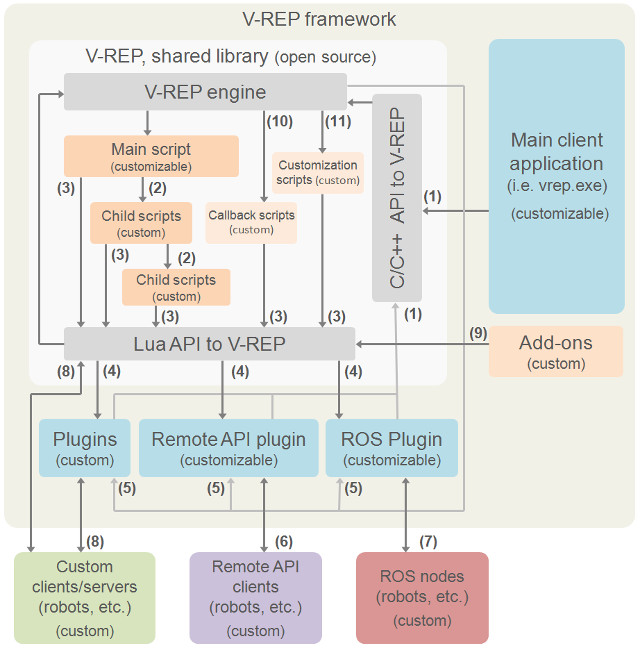
\includegraphics[scale=0.45]{vrepStruct.jpg}
     \end{center}
      \caption{Structure of the VREP-framework \url{http://www.coppeliarobotics.com/helpFiles/en/images/writingCode1.jpg} 13.10.2015 \label{fig:vrepStruct}}
    \end{figure}
    
    The V-REP main client application provides the basis vor the simulation. 
    V-REP bases on scenes in which the simulation settings and scenes are saved. 
    To run a simulation, the necessary objects need to be added to the scene. 
    An object can be a dummy object with no physical properties, a 3-D shape either imported via an .stl-file or created directly in V-REP. 
    V-REP already provides a library of objects, starting with sensors and continuing with whole robots. 
    An example are force sensors which can be used to connect object. 
    Then, the force sensor transmits the resulting forces and torques during the simulation and can be set to break when exceeding a certain threshold. 
    Connecting objects without force sensors can be used to separate physical simulation and visual representation. 
    The connection becomes static, so a complex, but visually appealing mesh shape can be attached to a simpler shape with appropriate physical parameters. 
    Thereby, physical simulation calculation are performantly done on the simple, and as V-REP provides several visibility layers, the user sees only the complex shape.
    
    V-REP provides several possibilities to extend the simulation programmatically. 
    The easiest and best integrated way are Lua-scripts. Lua scripts can be attached to simulation objects and are handles within the simulation environment. 
    When choosing non-threaded child scripts, they get executed every simulation step and can influence scene objects via a comprehensive API. 
    A V-REP simulation step consists of several sections. 
    To execute parts of the script only at certain points, the current simulation status can be checked before executing code.  
    The downside of these Lua-scripts is, that they are stored inside the binary scene file. 
    Thus, it's difficult to put them under version control or do collaborative work. 
    As the Lua-Engine inside V-REP provides full Lua support, this can be avoided by using the internal scripts only to import and call the actual scripts that are stored outside the scene. 
    In section \ref{sec:implSoftware} is described how we handled this problem in detail.
    
    If Lua doesn't offer the needed performance or functionalities, the second way to build deeply integrated software is the internal C++ API for plugins.
    The most flexible, but least performant way is the remote API of V-REP.
    Providing an API for Java, Matlab, Python and Urbi, it interacts with many programming languages.
    However, the functionality provided by the remote API is limited compared to the internal API for Lua or C++.
    For the remote API, V-REP needs to start a server that the client connects to.
    This is also possible over network, so the computation load can be distributed between different machines.
    
    For communication inside V-REP, global custom variables can be used. As the access to those is not supported by the remote API, a more flexible way are \emph{Signals}. \emph{Signals} can be of String, Integer or Float type and are globally accessible  in the current scene. 
    
    


    
    
    \section{Communication V-REP-Quadrocopters}
    \label{sec:comm}
    \textbf{\textit{Goal}:} our mixed reality simulation needs a dependable link of communication between the V-REP simulation environment and the flying quadrocopters. 
    The Quadcopter needs to stream its telemetry data in real-time to the V-REP, and the reverse communication is needed as well.\\
    The simulated quadrocopters that we have in the V-REP are divided into two categories: real and virtual representations.\\ 
    The real are replicating the physical flying quadrocopters. They should perform the same flying manoeuvres as those flying in the real environment. 
    In order to make the model replicate this behaviour, the flying quadrocopter must send its linear and angular velocity, its pitch yaw and row and other parameters in real time to its representation model in V-REP. 
    The simulation model should also send the readings from its proximity sensors to the flying quadcopter thus providing it with information from a virtual sensor. \\
    The virtual quadrocopters are purely simulation quadcopter objects, that exist only in the V-REP simulation environment. Their purpose is to interact with the real quadrocopters for example to avoid collisions and thus making the first steps in the swarm research. The virtual quadrocopters have to be seen in the Paparazzi ground station as if they are real physical quadrocopters. It means that all the ground station agents like message logger, the signal plotting, attitude indicator, artificial horizon and other displays have to be updated with adequate information coming from the virtual quadrocopters in the V-REP.
    
    The communication between the V-REP quadrocopter models and the physical quadrocopters passes through several software components, which are depicted on figure \ref{fig:communication} and discussed in the next chapters.
    
    \begin{figure}[h!]
     \begin{center}
      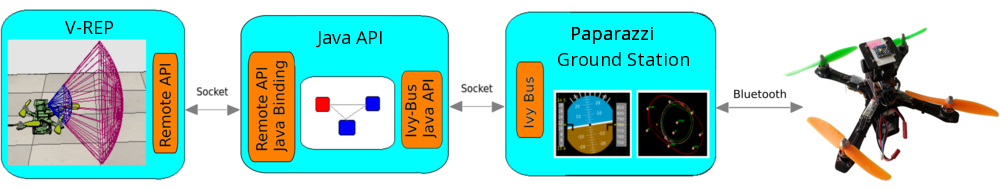
\includegraphics[scale=0.15]{communication.png}
     \end{center}
      \caption{communication V-REP - Quadrocopter\label{fig:communication}}
    \end{figure}
    
\subsection{V-REP Remote API}
    V-REP provides several means of communication with an external application. One of them is the Remote API, which allows to control a simulation (or the simulator itself) from an external application or a remote hardware (e.g. real robot, remote computer, etc.). The V-REP remote API is composed by approximately one hundred functions that can be called from a C/C++ application, a Python script, a Java application, a Matlab/Octave program, an Urbi script, or a Lua script. The remote API functions are interacting with V-REP via socket communication in a way that reduces lag and network load to a great extent.
    
\subsection{Java API}
    Java API is the external program, that we have implemented to communicate with V-REP through the Remote API.
    We have chosen to implement our external program, communicating with the V-REP, in the Java programming language regarding the following advantages: Java's platform independence allows to run the external program even on different machine with different operating system than the one used for running the V-REP environment.  Java is object-orientated which favours the use of design patterns and highly abstraction layers, which allows us to write an API that is modular, reusable and can later be easily extended to support other mixed-reality scenarious. Java also associates documentation with the actual code. The JavaDoc produces browsable documentation from the comments written in the code, which will be useful for anybody who wants to extend the project\\
    The implementation and architecture of the Java API is duscussed in details in \ref{sec:implementation}. The purpose of the Java application is to serve as a communicating bridge between the Paparazzi Ground Station and the V-REP. It detects all quadrocopters in the V-REP simulation, builds their virtual representations and feeds the models with real-time data.
    
\subsection{Ivy Bus}
    Ivy Bus is a simple protocol and a set of open-source (LGPL) libraries and programs that allows applications to broadcast information through text messages, with a subscription mechanism based on regular expressions. Ivy libraries are available in C, C++, Java, Python and Perl, on Windows and Unix boxes and on Macs. \\
    The Paparazzi Ground Station uses the Ivy Bus as a means of communication between the different software components. Figure \ref{fig:paparazziGS} depicts the communication structure in the Paparazzi Ground Station, in which the different agents communicate with each other by sending messages on the Ivy-Bus.
    
    \begin{figure}[h!]
     \begin{center}
      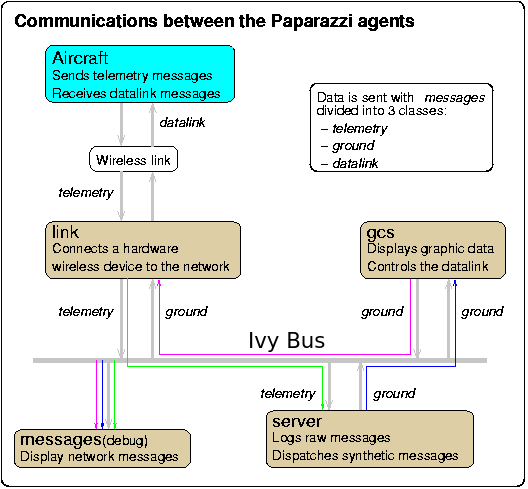
\includegraphics[scale=0.7]{paparazzi_gs.png}
     \end{center}
      \caption{Ivy-Bus in Paparazzi Ground Station\label{fig:paparazziGS}}
    \end{figure}
    
    The UAV (in blue) is streaming its telemetry data to the ground control station, which is received by the link. The \textbf{link} agent manages the ground-based radio modem and distributes the received messages to the other agents across the Ivy-Bus.
    
    The Ivy Bus is an example of a publisher-subscriber protocol, in which senders of messages, called publishers, does not  explicitly specify the address of the receiver, but just send the message on one, shared by all nodes, bus. The recipients, called subscribers, which are interested in the message will accept it and the others will ignore it. The publisher-subscriber is a many to many communication model in which publishers are loosely coupled to subscribers - there is no space, flow and time coupling. This means that the publishers does not have to know the addresses of the subscribers and even does not need to know of their existence. Each can operate normally without the other and can continue its thread of execution regardless if the subscriber has received the message or not. It also provides scalability, which means that we can “attach” our Java API to the Ivy-Bus and start publishing and listening for messages without changing any line of source code in the Paparazzi Ground Station software.
    
    In the publisher-subscriber model, subscribers typically receive only a subset of the total messages published. The process of selecting messages for reception and processing is called filtering. There are two common forms of filtering: topic-based and content-based.
    In a topic-based system, messages are published to "topics" or named logical channels. Subscribers in a topic-based system will receive all messages published to the topics to which they subscribe, and all subscribers to a topic will receive the same messages. The publisher is responsible for defining the classes of messages to which subscribers can subscribe.
    In a content-based system, messages are only delivered to a subscriber if the attributes or content of those messages match constraints defined by the subscriber. The subscriber is responsible for classifying the messages. Both filtering techniques are depicted in figures \ref{fig:pubsubsc_topic_based} and \ref{fig:pubsubsc_content_based}.
    
    The Ivy Bus is a content-based publisher-subscriber and uses regular expressions for the message filtering.
    
    \begin{figure}[!tbp]
      \centering
      \begin{minipage}[b]{0.4\textwidth}
        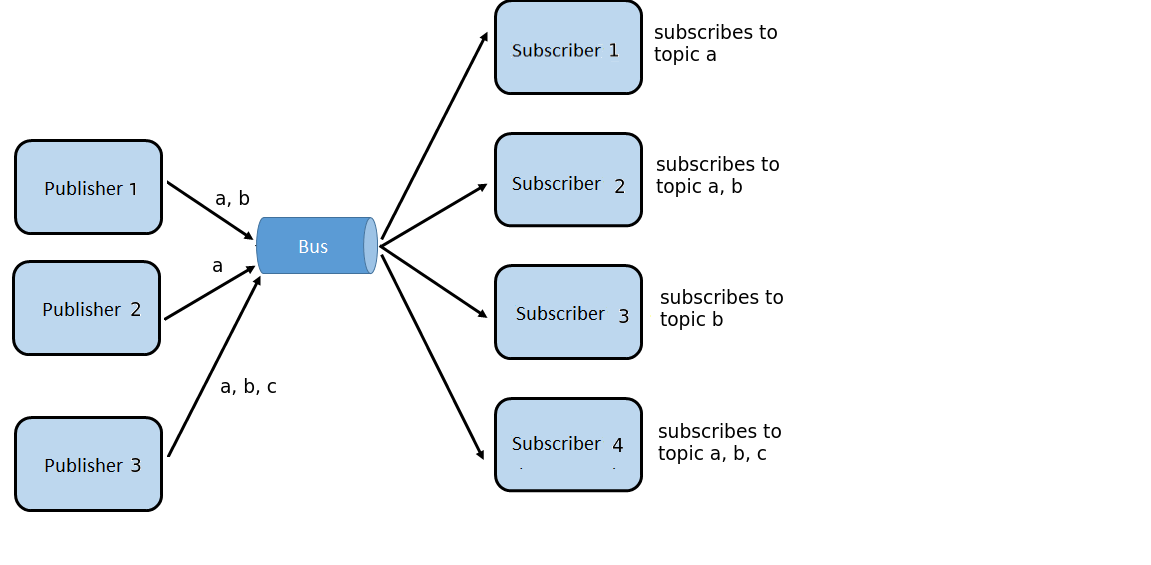
\includegraphics[scale=0.4]{pubsubsc_topic_based.png}
        \caption{Topic-based publisher-subscriber \label{fig:pubsubsc_content_based}}
      \end{minipage}
      \hfill
      \begin{minipage}[b]{0.4\textwidth}
        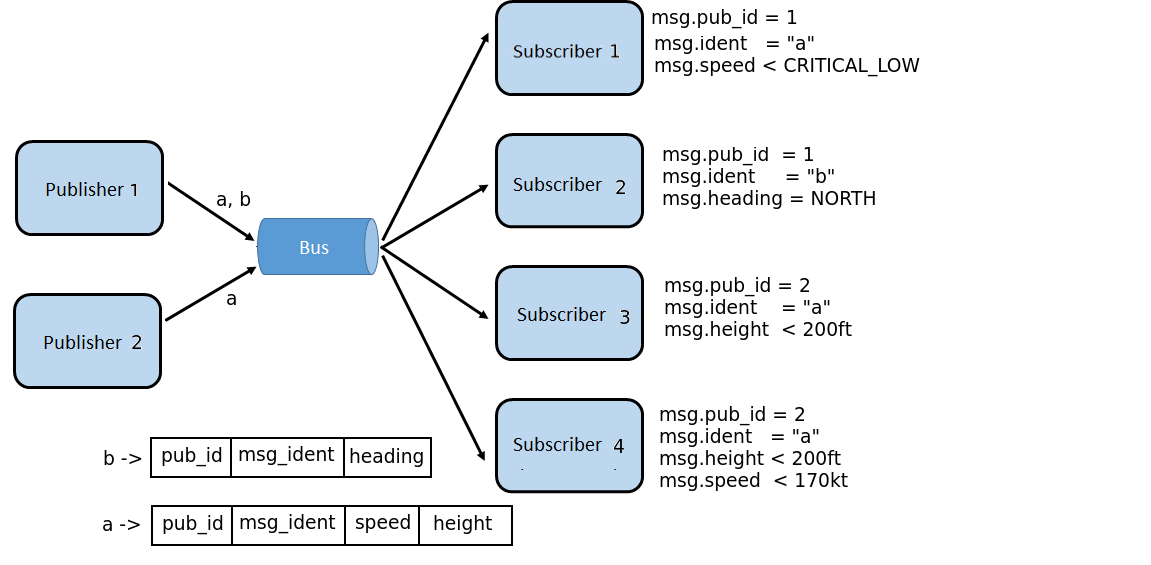
\includegraphics[scale=0.4]{pubsubsc_content_based.png}
        \caption{Content-based publisher-subscriber \label{fig:pubsubsc_topic_based}}
      \end{minipage}
    \end{figure}
    
    \subsection{Communication}
    \label{sec:communication}
    
    The communication between V-REP and the quadrocopters passes through the Java API, which serves as a bridge between them. In fact the Java API does not communicate directly with the quadrocopter, but connects to the Ivy-Bus in the Paparazzi GS and can thus subscribe to the messages caring the telemetry data and also publish messages which will eventually be send to the quadrocopter by the link agent. On the other hand it uses the V-REP Remote-API to exchange information and provide the V-REP quadrocopter models with the data retrieved from the Ivy-Bus messages.\\ 
    Since we wanted to create a modular and reusable API, that can be used for other mixed-reality scenarios, the Java API was created with the idea in mind to be distributed, modular and rely on many abstraction layers.\\ 
    The API development has followed the requirement-driven principles and its main tasks are described in the following paragraphs. The implementation of the described bellow requirements in described in \ref{sec:commImplementation} of \ref{sec:implementation}.
    
    \subsubsection{V-REP-Remote API specific requirements}
    \label{sec:requirementsVREP}
    
    Below is a description of the requirements for the Java API which is responsible for the connection and communication with the V-REP environment. Its implementation is described in \ref{sec:vrepImplementation} of \ref{sec:implementation}.
    
    \paragraph{Connection to V-REP through the Remote API}
    
    There should be implemented a mechanism that enables to establish connection to the V-REP simulation. The connection should be able to be disconnected and reconnected at any time. Since the Remote API is based on a socket connection, it should be possible to connect to a V-REP server, situated on another machine, by specifying its IP address and port number. This will allow to run the V-REP simulation on a remote, powerful computer and thus release the local computer from having to deal with the simulation and communication program at the same time.
    
    \paragraph{V-REP scene object and scene representation}\label{sceneobject}
    \todo{integrate into sectionsec:theoryVrep}
    The main elements in V-REP that are used for building a simulation scene are scene objects (objects in short). Objects are visible in the scene hierarchy and in the scene view. In the scene view, objects have a three dimensional representation. Some of the object types are: shape, joint, proximity sensors, vision sensors and others. The shape object is a rigid mesh that is composed of triangular faces. Our quadrocopters are represented as a shape objects in the V-REP scene. But is also contains four infrared sensors which are of type proximity sensor object. So the quadrocopter is represented as a complex scene object. 
    The V-REP scene objects have to be represented as individual classes in order to be able to easily distinguish them and work with their properties. The class representing the scene object must have as fields the properties describing the simulation object - liniar and angular velocity, position and orientation. The V-REP scene object hierarchy should also be implemented by using inheritance and composition object oriented techniques. \\
    The Java API should provide methods to retrieve all scene objects from the V-REP scene and store them in a virtual scene representation for later use.\\
    Since our quadrocopters are represented as shape objects and typically a V-REP scene contains at least 20 shape objects by default, there should be implemented a scanner that retrieves the quadrocopters from the scene. The scanner must be able to retrieve the virtual and real quadrocopters in a separate containers.
    
    \paragraph{Continuous data exchange between quadrocopter instances and V-REP}
    
    As mentioned at the beginning of \ref{sec:comm} we divide our quadrocopters in virtual and real representation. The virtual representations exist only in the V-REP scene, but they have to be visible in the paparazzi ground station as if they are real flying drones. It means that all the quadrocopter flying parameters have to be sent to the paparazzi ground station as messages. It becomes clear that the virtual quadrocopters have to be provided continuously with live data from the V-REP - linear/angular velocity, position and orientation. The real quadrocopter representations does not need to be provided with V-REP parameters, since its velocity, orientation and height are coming from the physical flying drone, but it has to be provided with data from its proximity sensor scene objects. The update with V-REP data should have a frequency equal to the simulation step used - 50 ms by default.\\
    The real quadrocopter representation get provided with velocity, orientation and height from the physical flying quadrocopter and this data have to be provided to the V-REP quadrocopter object in order to fly like the physical one. This is the inverse communication from quadrocopter to V-REP and is realized with V-REP signaling mechanism. The update is done each time a new message has been received by the physical drone and its frequency depends on how often the messages are streamed from the copter and the communication latency. In order to achieve a realistic flying manuevers and have minimum drift the update should not exceed 20 ms.
    
    \subsubsection{Ivy Bus specific requirements}
    \label{sec:requirementsIVYBus}
    \paragraph{Ivy Bus connection}
    Each participant which wants to exchange information on the Ivy-Bus is described as a singular and independent bus node. In our program the participants that want to exchange data on the Ivy-Bus are the virtual and real representations of the quadrocopters. There should be designed a class, which allows the connecting on the bus, publishing and subscribing to messages. The quadrocopter representations have to inherit from it or composite it and thus become independent bus nodes.
    
    \paragraph{Message retrieval and subscription}
    \label{par:messageRetrieval}
    
    All the messages that the paparazzi software uses are described in a xml file called \textit{messages.xml}, residing in the \textit{/paparazzi/conf/} directory. The following listing is an example of the messages file containing two messages.
    
    \begin{lstlisting}[basicstyle=\tiny, caption={Message Xml definition}, label={lst:MessageXml}, language = Xml]
    <msg_class name="telemetry">
     <message name="AIRSPEED" id="54">
        <field name="airspeed" type="float" unit="m/s"/>
        <field name="airspeed_sp" type="float" unit="m/s"/>
        <field name="airspeed_cnt" type="float" unit="m/s"/>
        <field name="groundspeed_sp" type="float" unit="m/s"/>
      </message>
      
      <message name="SONAR_ARRAY" id="216">
    	<field name="sonar_front" type="uint16" alt_unit="cm"/>
    	<field name="sonar_right" type="uint16" alt_unit="cm"/>
    	<field name="sonar_back" type="uint16" alt_unit="cm"/>
    	<field name="sonar_left" type="uint16" alt_unit="cm"/>
      </message>
    	
    	  . . . . 
    	  
    </msg_class>
    \end{lstlisting}
    
    In order to make the subscription and publishing of messages on the bus easier, each message should be represented as a corresponding class containing the message fields with its type and units.
    
    There should be implemented a class, which reads the \textit{messages.xml} file and creates an instance of the message class for each message. \\
    Once the messages are retrieved, the Ivy-Bus node should be capable of subscribing and publishing of any of the retrieved messages. The subscription should by dynamic and allow to subscribe to a new messages even at runtime. \\
    Once a message has been received, the Ivy-Bus node should provide the instance of the received message and its fields should contain the actual sensor values.\\
    Since our mixed reality scenario can involve many flying quadrocopters, there will be published the same messages but from different copters. In this case the messages are identified with the drone id number.
    Another requirement is that the Ivy-Bus node have to subscribe just to the messages published from the copter that it was assigned to and not receive the same messages from the other copters.
    
    \subsubsection{Application specific requirements}
    \label{sec:requirementsApplication}
    
    \paragraph{Aircraft retrieval}
    The paparazzi software stores important information about the quadrocopters in an Xml file stored in \textit{/paparazzi/conf/conf.xml}
    
    \begin{lstlisting}[basicstyle=\tiny, label={lst:AircraftXml}, language = Xml]
      <conf>
        <aircraft
          name="Quad_Lia_ovgu_01"
          ac_id="1"
          airframe="airframes/ovgu/free_flight.xml"
          radio="radios/spektrum.xml"
          telemetry="telemetry/ovgu/tmp_christoph.xml"
          gui_color="white"
        />
        
        <aircraft
          name="Quad_Lia_ovgu_02"
          ac_id="2"
          airframe="airframes/ovgu/free_flight_flow.xml"
          radio="radios/spektrum.xml"
          telemetry="telemetry/ovgu/free_flight.xml"
          gui_color="#b34c14805f44"
        />
      
      </conf>
    \end{lstlisting}
    
    Each quadrocopter is described as an aircraft, which has its name, id and other attributes. The parameter that is of specific importance for us is the id number, which is added to each message sent by the quadrocopter. The content based filtering of the messages is based on this aircraft id number. It is required to create a XML reader that parses the XML document and returns an instance of each aircraft class for each aircraft entry in the XML file.
    
    \paragraph{Virtual and Real Quadrocopters representation}
    
    The virtual and real quadrocopters have to be described by an appropriate class. \\
    Since they contain shared data and properties, an abstract parent class representing the quadrocopter will be an appropriate solution. The abstract quadrocopter should contain the aircraft it belongs to, so the name of the quadrocopter will coincide with the name of the aircraft. 
    Since the id of the aircraft it represents is also contained, the quadrocopter will be able to send and receive the messages that only belong to the quadrocopter it represents. \\
    Since the abstract quadrocopter represents also a V-REP scene object itself, it should contain the \textit{Shape} object it represents. Thus the orientation, rotation and velocity of the quadrocopter will be retrieved directly from the \textit{Shape} object.\\
    The proximity sensors of the quadrocopters should also be modelled and the abstract quadrocopter should provide methods to retrieve the distances measured by the sensors.\\
    The abstract class should also contain an IvyBus node, discussed in \ref{sec:requirementsIVYBus}, which will allow to connect/disconnect the quadrocopter from the IvyBus and to send and subscribe to messages filtered by the aircraft id it has. \\
    In general the abstract quadrocopter should be a highly polymorphic class, being a scene object, aircraft and IvyBus node at the same time. 
    It should have an interface allowing to connect/disconnect from the IvyBus, return object name, position, orientation, velocities and proximity sensor values. \\
    The real and virtual quadrocopters have to be subclasses of the virtual one, implementing their specific behaviour. 
    For example the real quadrocopter subscribes to the messages coming from the quadrocopter it represents and on message arrival retrieves the relevant parameters like pitch, yaw, row, thrust and updates the V-REP model using the signals mechanism. 
    The virtual quadrocopter on the other hand takes the parameters from the scene object, that is represents, packs them in messages with the id of the aircraft it represents and publishes them on the IvyBus.
    
    \paragraph{Real and Virtual Quadrocopter retrieval}
    
    There should be implemented an automatic mechanism, that retrieved the instances of the real and virtual quadrocopters. The retrieval should be based on the scene objects retrieval and the aircraft parsing introduces in the previous paragraph. \\
    After getting a list of all V-REP scene shape objects and all Aircrafts, it could be iterated in both lists and checked if any of the shape object's names matches the name of an aircraft. If the names match there should be created an instance of virtual or real quadrocopter with the corresponding Shape and Aircraft objects.
    The decision if it is a real quadrocopter or a virtual one depends on the object name. The real quadrocopters have the standard FINKEN drone names like \textit{\texttt{Quad\_Lia\_ovgu\_01}}, \textit{\texttt{Quad\_Lia\_ovgu\_02}} and the virtual have an arbitrary name with s prefix \textit{Virtual}.

% example for definition    
% \begin{definitionnonum}[Softwarearchitektur ]
% Die Softwarearchitektur repräsentiert alle Softwarekomponenten und deren Interaktionen in einer hierarchischen Struktur. Es werden sowohl statische Aspekte wie Schnittstellen und Datenpfade zwischen Softwarekomponenten, als auch dynamische Aspekte wie Prozessabläufe und zeitliches Verhalten beschrieben.
% \end{definitionnonum} 
 

  
%  example for bulletpoints
%\begin{itemize}    
%	\item{(überarbeiteter) Sicherheitsplan nach ISO 26262-6:2011, 5.5.1}
%	\item{Design- und Programmierrichtlinien für Programmier- und Modellierungssprachen nach ISO 26262-6:2011, 5.5.5}
%	\item{Hardware-Software-Interfacespezifikation nach ISO 26262-4:2011, 7.5.6}
%	\item{Software-Sicherheitsanforderungen nach ISO 26262-6:2011, 6.5.1}
%	\item{(überarbeiteter) Software-Verifizierungsplan nach  ISO 26262-6:2011, 6.5.3}
%	\item{Software-Verifizierungsbericht nach ISO 26262-6:2011, 6.5.4}
%\end{itemize}

 
%example for table    
% \begin{table}[h]
%      \centering
%    \caption{7.4.1 Notationen für Softwarearchitekturen\cite{iso6}}
%    \begin{tabular}{|c|l|c|c|c|c|}
%      \hline
%     \multicolumn{2}{|c|}{\multirow{2}{*}{Methoden}} & \multicolumn{4}{|c|}{ASIL}\\
%      \multicolumn{2}{|c|}{} &A & B & C & D\\
%      \hline
%       1a & Informelle Notationen & ++ & ++ & + & +\\
%      \hline
%       1b & Semi-formale Notationen & + & ++ & ++ & ++\\
%      \hline
%        1c & Formale Notationen & + & + & + & +\\
% 
%      \hline
%      \end{tabular}
%      \label{tab:archDescr}
%\end{table}

\ifgerman{\chapter{Auswertung}}{\chapter{Implementation}}
\label{sec:implementation}

\section{Simulation Environment}

The FINken consists of the body, the rotors and the sensors. The body contains the behavioural and flight control, the thrust simulation is handled by scripts connected to the rotor structure.

\subsection{Scene Modeling}

The body consists of multiple objects, while visual representation and the physical behaviour are split. For visual representation, a *.stl file from the CAD-Model of the original FINken was imported. This shape is rather complex, which makes the simulation time consuming. To speed up the simulation, the shape of the finken was remodelled in VREP, using only simple rectangular shapes. Making the complex shape static, establishing a fixed connection and hiding the simple shape, the result is a a visual appealing simulation object with good simulation performance. A dummy-object is used as a singular measurement reference point in the middle of the FINken. This has to be taken into account when targeting physical objects, as the FINken will not be able to reach the target completely without colliding with the object. This dummy object should always be used when refering to the FINkens position, orientation or movements, as it is aligned to the global coordinate system while especially imported shapes may be rotated in the simulation. Vrep provides several pre-configured sensor type, the real FINkens sensors were modeled by using existing ultrasound distance sensors. The FINken is equipped with Maxbotix MB1232: I2CXL-MaxSonar-EZ3 sensors\url{(http://www.maxbotix.com/documents/I2CXL-MaxSonar-EZ_Datasheet.pdf}). According to the datasheet, they have an opening angle of $\angle{30}$ at maximum range when detecting smaller objects and maximum range of 7.65m for larger objects as walls. The datasheet states a rather complex beam shape, but for the simulation a cone with an opening angle of $\angle{30}$  and a height of 7.65m will be used. Finally, a dummy target objects belongs the virtual FINken. This object can be moved manually in the scene and the simulated quadcopter will fly towards it.  As the real FINken doesn't have the ability to fly to predefined points, we only used this feature for development.

\begin{figure}[h!]
 \begin{center}
  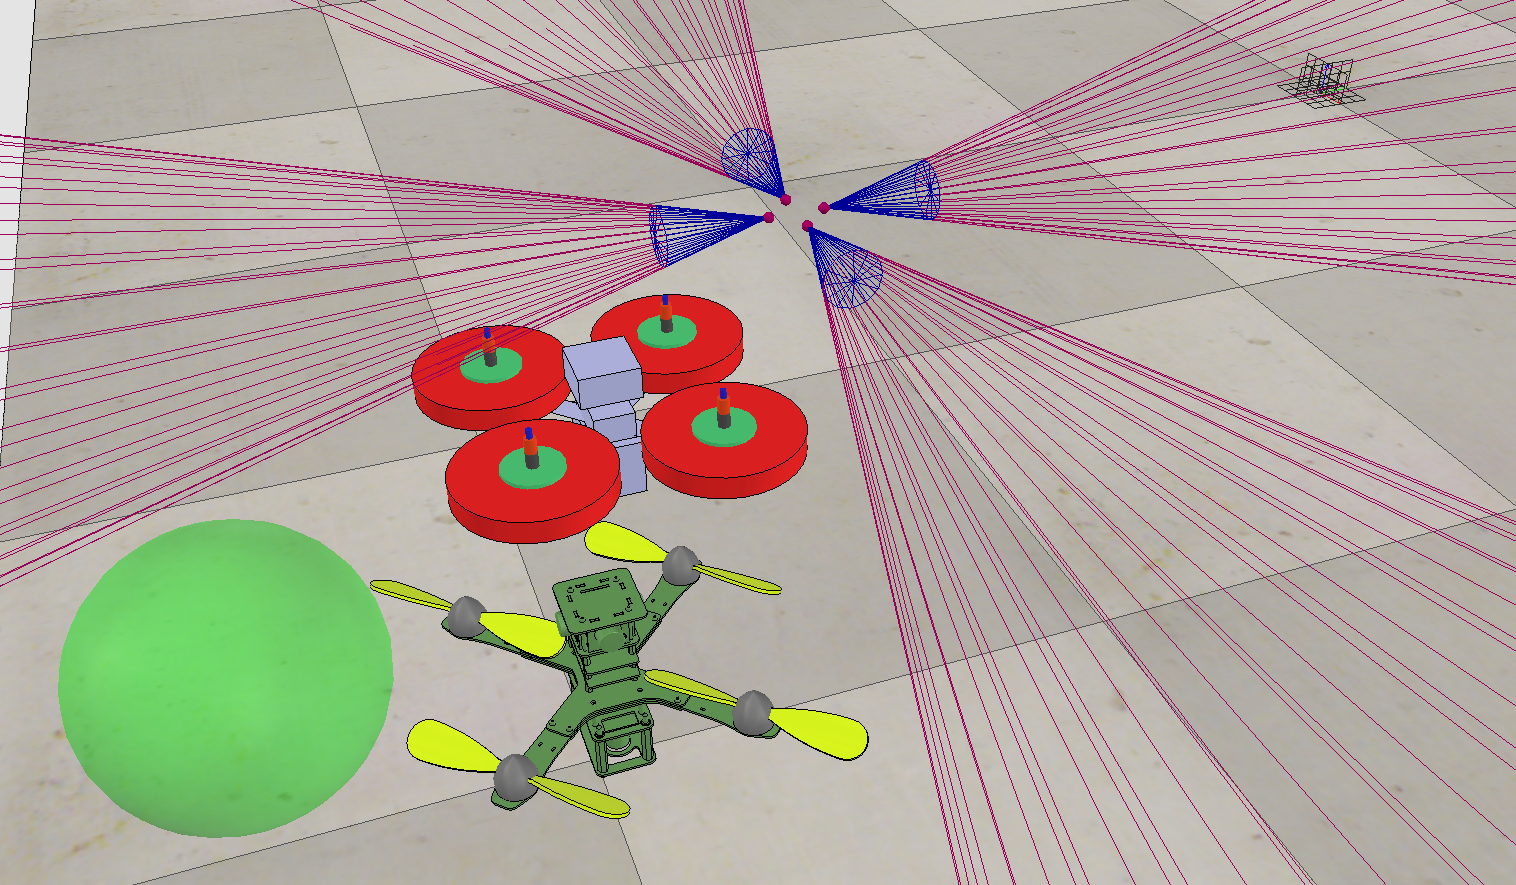
\includegraphics[width=\linewidth]{vrepDisassemlbyFull.png}
 \end{center}
  \caption{Parts of the simulation object \label{fig:vrepParts}}
\end{figure}

The measured weight of the real FINken was applied to the simulation object. As no advanced modelling like calculating moments of inertia was done, the weight of the motor was applied separately to the rotor model in VREP.  The motor assembly adds significant weight outside the FINkens center of gravity and therefore has a rather large influence on its behaviour. 
\todo{weight table for finken2 and finken3}
The linear damping factor of the FINken body material was set to 0.3, to decrease drift and to model the air resistance of the real FINken, which is minimal but nevertheless existent.


The rotor model in VREP handles the thrust simulation and thus a huge part of the physical behaviour of the quadcopter model.  Again, visual representation and physical simulation are separated. 
\todo{add picture of rotor}
The visualisation is done with a static shape of a rotor, that is connected to a joint and rotates with a fixed speed. During flight, the rotation speed does not really change visually noticeable, a dynamic adaption of the rotation would only increase computation time without much benefit. Of course, the rotor shape could be made non-static and rotate in a particle stream, and apply the thrust force according to the particle collisions, but again, this would mean a massive increase of computation power and is not needed for our purposes.

\begin{figure}[h!]
 \begin{center}
  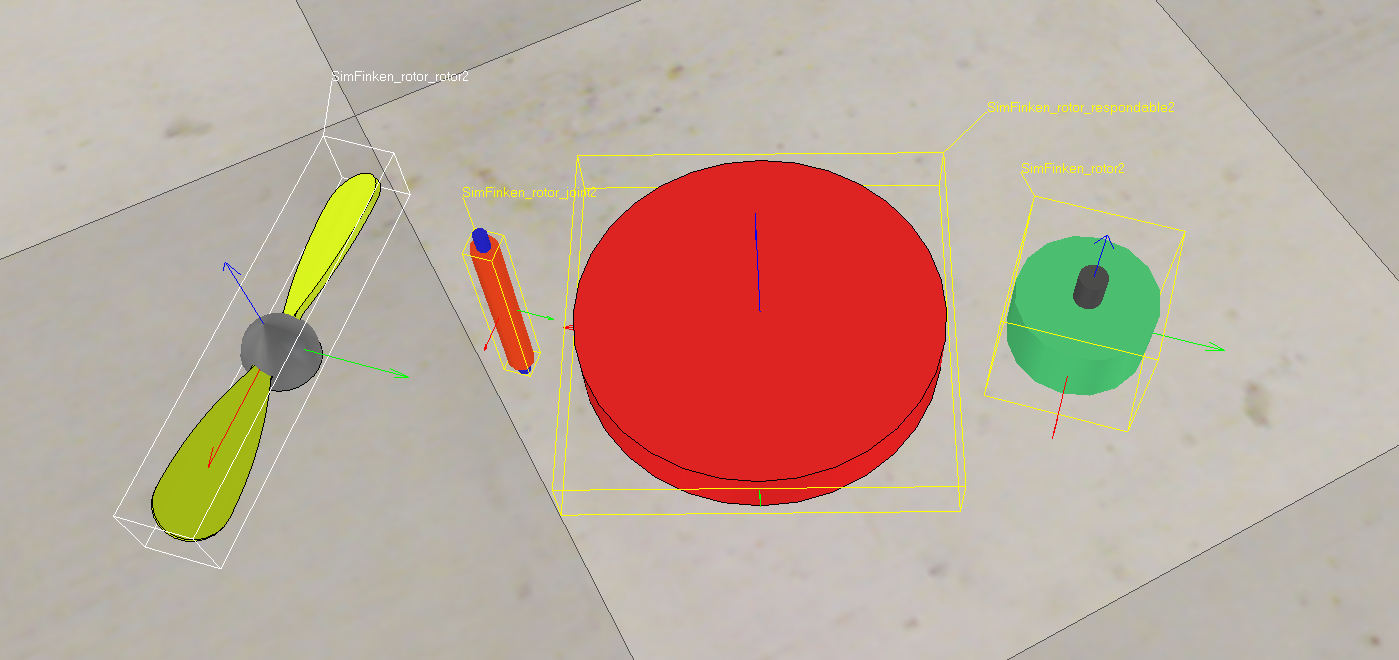
\includegraphics[width=\linewidth]{vrepRotorLegend}
 \end{center}
  \caption{Parts of the simulated rotor \label{fig:vrepRotor}}
\end{figure}


The rotor model is attached to the FINken body via a force sensor which applies the forces and torques calculated in the physical rotor model to the FINken body. The rotor is represented by a cylindrical shape which resembles the area swept by a real rotor and uses a particle simulation to emulate the airstream. The handling of the particle simulation is done inside a lua child script attached to the rotor model. The script has several parameters for the particle simulation, \todo{add complete param list}.
During simulation, the particle velocity is the parameter used to control the finken. This rotor model was already included in VREP as an example and was used without further modifications, the theory behind it is shortly explained in \ref{sec:theomodel}. Using the particle simulation has the advantage of providing a small random factor that causes noise and it simulates the airstream which will influence  other copters in multicopter scenarios.



\subsection{Flight controller in simulation}

The V-REP example quadrocopter already included some flight controller out of the box

\begin{itemize}
\item{PID implementation with I-reset}
\item{}
\item{}
\item{}
\end{itemize}
\todo{finken parameter estimation}

\todo{controller tuning}


\begin{table}[h]
	\centering
	\begin{tabular}{|c|c|}
    		\hline
		Parameter & Value \\
		\hline
    		Physics engine & Bullet\\
    		\hline
    		Dynamics settings & Accurate (default) \\
    		\hline
    		Simulation time step & 50 ms (default) \\
    		\hline
    		Real-time mode & enabled \\
    		\hline
	\end{tabular}
    	\caption{V-REP simulation parameters}
      	\label{tab:simSettings}
\end{table}

\subsection{Simulation Software Structure}

\todo{finish diagram of finken software}
\tikzset{
    group/.style={
           rectangle,
           rounded corners,
           draw=black, very thick,
           minimum height=2em,
           inner sep=2pt,
           text centered,
           },
           swScript/.style={
           rectangle,
           draw=black, very thick,
           minimum height=2em,
           inner sep=2pt,
           align = left,
           },
           vrepObject/.style={
           circle,
           draw=black, very thick,
           minimum height=2em,
           inner sep=2pt,
           text centered,
           },
           vrepEnv/.style={
           ellipse,
           draw=black, very thick,
           minimum height = 5cm,
           minimum width = 3cm,
           },
            implements/.style={
            -{open triangle 60}, dashed
           },
           inherits/.style={
           -{open triangle 60},
           }
}
\begin{figure}[h]
	\centering
	\begin{tikzpicture}[scale=2, node distance = 1cm, auto]
		%vrep part
		\node[vrepEnv](vrep){};
		\node[below=0.3cm of vrep.north]{\underline{V-REP}};
		\node[vrepObject, below =1.1cm of vrep.north](fink1){finken1};
		\node[vrepObject, below =0.4cm of fink1.south](fink2){finken2};
		%lua script part
		\node[swScript, rectangle split, rectangle split,rectangle split parts=3, right=of vrep.45](finkenMeta){finkenMeta\nodepart{second}
			public:
			\nodepart{third}
			public: \\
			step() \\
			sense() };
		\node[swScript, rectangle split, rectangle split,rectangle split parts=3, below=of finkenMeta](finken){finken\nodepart{second}
			public:
			\nodepart{third}
			public: \\
			step() \\
			sense() };
		\node[swScript][rectangle split, rectangle split,rectangle split parts=3, right=of finken](finkenCore){finkenCore 
			\nodepart{second}
			public:
			\nodepart{third}
			public: \\
			step() \\
			sense()}; 
		\node[swScript, rectangle split, rectangle split,rectangle split parts=3, above=of finkenCore](finkenPID){finkenPID\nodepart{second}
			public:
			\nodepart{third}
			public: \\
			init(P,I,D) \\
			step(error, $\delta$t) };
		%connections
		\draw[inherits] (finken) to (finkenCore); 
		\draw[-{angle 60}](finkenCore) to (finkenPID);
		\draw[implements](fink1) to (finken);
		\draw[implements](fink2) to (finken) ;
		\draw[implements](vrep.45) to (finkenMeta);
	\end{tikzpicture}
	\caption{Software structure of the FINken Simulation}
	\label{fig:finkenSoftStruct}
\end{figure}

The simulation software is written in Lua and runs inside a non-threaded child script of each FINken quadrocopter in VREP.  

The base class is the finkenCore, which contains the main flight control algorithm and a steering interface as well as an interface to the FINkens sensors.
The input commands for controlling the FINken are set via the signal communication of VREP. Signals inside VREP are the most versatile communication possibility which can be accessed from anywhere inside VREP and any remote API, they can be seen as a kind of global variable. Signals can be of integer, float or string type, where custom data types can be sent in text form as string signals. 

The finkenCore needs to be initialized at simulation start the for each simulated FINken. It starts the VREP remote API server and creates the API signals. Also, the PID controllers for flight control are initialized. 
During simulation, calling the FINkenCore.step() method handles the flight control. The input values are read from the signals \textit{pitch}, \textit{roll}, \textit{yaw} and \textit{throttle}. When the signal \textit{height} has a positive value, the FINkenCore will control the thrust so that the simulated FINken will keep the height provided by the signal, otherweise only the \textit{throttle} signal is used directly. The previously initialized PID controllers are used to compute the target air stream velocity for each rotor to move the simulated FINken to the target orientation.

To keep a quadcopter at a certain height without an external reference requires an exact equilibrium between gravity and thrust. The current real FINkens do not compensate the battery voltage, so the same throttle corresponds to different thrust forces during flight. Also, each FINken unit has slightly different base thrust. Therefore, the thrust in the simulation is tuned with a logisitc curve \ref{equ:logistic} to decrease the influence of the throttle close to the hover thrust. 
\begin{equation}
throttle_{tuned} = \begin{cases}
-\frac{a * |throttle|}{a - |throttle| + 50} + 50 & throttle < 0 \\
\frac{b * throttle}{b - throttle + 50} + 50 & throttle >= 0\\
\end{cases}
\label{equ:logistic}
\end{equation}
The default values for the throttle tuning function are  $a = 1$ and $b = 1$. 
\todo{insert plot of function?}


The simulated FINken is equipped with 4 distance sensors which resemble the 4 ultrasound sensors of the real FINken. The FINkenCore module contains a \textit{sense()} function that reads the 4 distance sensors and writes the values to the signal \textit{sensor\_dist}. As signals only support limited data types, \textit{sensor\_dist} is a string signal containing a packed float array. The array contains the distances in the order \textit{front}, \textit{left}, \textit{back}, \textit{right}.  If the FINken gets more sensors in the future, their evaluation has to be added to this method.
By writing the distance values to a signal, they can be propagated to the Ivy-Bus and thus to the real FINken by our Java communication app, which enables the real FINken to detect virtual objects, as simulated FINken or walls that only exist in the Simulation.


While the FINken is normally controlled by setting the pitch, roll, yaw and throttle directly, an alternative is to specify a target object. This method was originally used by the example quadcopter model of V-REP, though the function works differently in the FINkenCore now. When calling  \textit{setTarget(targetObject)}, the differences in x, y and z coordinates of the FINken base to the target objects are given to three PID controllers which calculate the pitch, roll and throttle to move the FINken to the target objects position. Those values are then published via the control signals for the FINken and regularly processed by it's internal controls. Therefore, \textit{setTarget(tragetObject)} needs to be called every time before \textit{step()}, when a target object should be approached.

In the previous sections, only the signal names for the first simulated FINken were used for better readability. As the simulation is scalable, more than one FINken can be added, therefore a naming scheme for signals is needed to prevent collisions of the globally visible signals. The signals corresponding to the first FINken are \textit{pitch}, \textit{roll}, \textit{yaw}, \textit{throttle}, \textit{height} and \textit{sensor\_dist}. For the second FINken, when the first one is copied, VREP automatically adds "\#0" to it's name. Following this convention, but leaving the '\#' to prevent problems with special characters when forwarding the signals through our interface, we add '0' to the signal names for the second FINken and consecutively enumerate following FINkens.

The finken.lua module provides an basic structure for further enhancements. It's contained functions like \textit{step()} and \textit{sense()} are called called inside V-REP during the appropriate simulation step sections. By calling custom functions inside those functions, the behaviour of the FINkens can be customised without any need to change the lua scripts inside V-REP. If a heterogenous swarm of FINkens with different functionalities should be implemented, the different finken-scripts have to be imported by the different FINkens in the simulation, which needs to be done in the lua scripts inside V-REP.


FinkenMeta.lua is loaded in the child script of a dummy object in the scene  to have an API to the simulation that is not connected to a single FINken. This can be used to dynamically manipulate the environment during simulation, e.g. by adding objects like other FINkens.
\section{Communication V-REP - Quadrocopters}
\label{sec:commImplementation}

This chapter describes the implementation of the requirements on the Java-API, which ware discussed in \ref{sec:communication} of \ref{chap:theo}. It begins with an overview of the software architecture and continues with the explanation of the created projects, classes and their use. It helps understanding how the communication between the V-REP and the quadrocopters is implemented and how to use the API or extend it in order to implement other mixed-reality scenarios.\\
Note that this is just a brief explanation of the Java-API implementation. If you want to go in details refer to the Javadoc which is also provided as an attachment to this paper.

\subsection{Software architecture}

The software architecture of the Java-API, which serves as a communication bridge between the Paparazzi software and the V-REP simulation, is designed to be as modular as possible in order to facilitate the further development of the project. Its reusable components should also serve as a building blocks for the students that want to develop future mixed-reality projects. \\

On \ref{fig:apiArchitecture} is depicted an raw overview of the Java-API software architecture.
The final program is assembled from independently developed components. Each part is independent and provide well-defined exported interfaces so that the other parts can use them.
The first layer contains the projects \textit{JavaV-REP}, \textit{JavaIvyBus} and \textit{JavaXmlSax}.\\
The \textit{JavaV-REP} is the implementation of the requirements concerning V-REP, that ware discussed in \ref{sec:requirementsVREP} of \ref{chap:theo}. At the heart of this project is the V-REP Remote-API binding for Java provided by Coppelia. The \textit{JavaVrep} project extends this library and provides further utility methods for establishing connection to remote V-REP servers as well as retrieving and manipulating scene objects. The \textit{JavaV-REP} project is described in more details in \ref{sec:vrepImplementation}.\\

\begin{figure}[h!]
 \begin{center}
  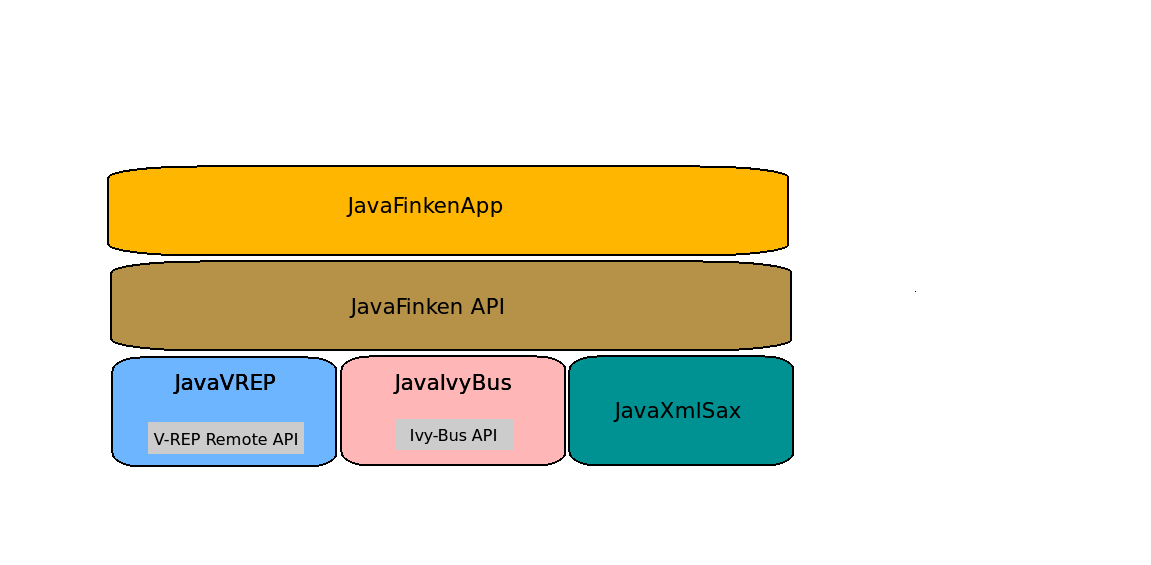
\includegraphics[scale=0.6]{apiArchitecture.png}
 \end{center}
  \caption{Java-API architecture\label{fig:apiArchitecture}}
\end{figure}

\textit{JavaIvyBus} is a Java project, that imports the Ivy-Bus library and implements the requirements regarding Ivy-Bus, which ware discussed in \ref{sec:requirementsIVYBus}.\\ 
It extends the functionality of the the Ivy-Bus library and provides the programmer with the possibility to create Ivy-Bus nodes by just instantiating an object which takes as constructor parameter the name of the bus-node. It facilitates the connection or disconnection from the bus by just calling a function the the created bus-node object. The abstractions on which this project rely also allow to easily create bus messages or just parse them from xml file and subscribe to them even dynamically. The \textit{JavaIvyBus} project is discussed in more detail in \ref{sec:ivyBusImplementation}. \\

The \textit{JavaXmlSax} project is a small API, that allows the programmer to easily create a custom xml reader that parses any xml document and retrieves the instances of the objects defined by the xml. It consists of several abstract classes, that provide the template for the custom xml readers.\\
A short explanation of how this API can be used is included in \ref{sec:xmlImplementation}. \\

On the next layer in the hierarchy is the \textit{JavaFinken} API. It uses the APIs from the layer below to provide further abstractions and utilities for our FINKEN project. It consists of classes that describe 
the aircrafts defined in the paparazzi, defines the basic classes that represent our virtual and real quadrocopters and their sensors, defines a representation of the telemetry and the V-REP signals. With the help of \textit{JavaIvyBus} API, lying on the layer below, the Ivy-Bus nodes, specific for the virtual and real quadrocopters are represented. The abstraction provided by \textit{JavaXmlSax} is used to create a custom Xml readers for parsing the telemetry, messages and aircrafts from the Xml files. A more detailed description of the API is included in \ref{sec:javaFinkenImplementation} \\

On the top of the hierarchy is situated the actual application of our project called \textit{JavaFinkenAPP}. It uses \textit{JavaFinken} API to bind the provided utility classes in a specific application meeting our project requirements. The application has a simple Graphical User Interface that facilitates specifying the IP and Port number of the V-REP simulation server, specifying path to the paparazzi software, a button for establishing the connection and other UI elements.




\subsection{JavaV-REP}
\label{sec:vrepImplementation}

All the functionality, that concerns V-REP and was discussed in \ref{sec:requirementsVREP} of \ref{chap:theo} is implemented as a single Java project called \textit{JavaVREP}.\\
 The project uses the V-REP Remote-API Java binding - package \textit{coppelia} (containing 12 Java classes) and the \textit{libremoteApiJava.so} or \textit{libremoteApiJava.dll} (depending if the platform is Linux or Windows). The \textit{libremoteApiJava.so} should be placed in the Java home directory, e.g \textit{/usr/lib/jvm/java-8-oracle/jre/lib/amd64}, in order for the project to be compiled.\\
The main class is the \textit{VrepConnection.java}, which is a wrapper of the \textit{remoteApi.java} class provided by the V-REP remote API. Its singleton instance can be retrieved by calling:

\begin{center}
\begin{tabular}{c}
\begin{lstlisting}[basicstyle=\small]
VrepConnection connection = VrepConnectionUtils.getConnection();
\end{lstlisting}
\end{tabular}
\end{center}

The above expression loads the remote API library and returns the instance of \textit{VrepConnection} on which the Remote API functions are called. For example to retrieve all objects in a scene the following function have to be called on the \textit{VrepConnection} instance:

\begin{center}
\begin{tabular}{c}
\begin{lstlisting}[basicstyle=\small]

connection.simxGetObjects();

\end{lstlisting}
\end{tabular}
\end{center}

The interfaces \textit{VrepServer} and \textit{VrepClient} and their implementations \textit{StandardVrepServer} and \textit{StandardVrepClient} describe the two end-points of the communication. The \textit{VrepServer} describes the IP address and the port number of the machine on which the V-REP is running. In order to connect to a V-REP server we have to create in instance of the \textit{VrepServer} and open the client:

\begin{center}
\begin{tabular}{c}
\begin{lstlisting}[basicstyle=\small, language=Java]
VrepConnection connection;
VrepClient     client;
VrepServer     server;

connection = VrepConnectionUtils.getConnection();
client     = VrepClientUtils.getClient();
server     = new StandardVrepServer("127.0.0.1", "19999");

client.connectToServer(server);

if (!client.isConnected()) {
// error in connection
} 
\end{lstlisting}
\end{tabular}
\end{center}

The above example shows how to connect to a V-REP server. The IP \textit{127.0.0.1} specifies that the server is running on the same machine. The port number can be chosen arbitrary, but have to match on both client and server site.\\
In order to close the connection just the method \textit{client.close()} has to be called. \\

The \textit{VrepClient} conforms to the Java Beans specification and can thus fire events when the connection has been established or disconnected. Any class who is interested in catching these events asynchronously, for example GUI, will have to implement \textit{PropertyChangeListener} and register. See
\url{https://docs.oracle.com/javase/tutorial/javabeans/writing/events.html} for more information. \\

Each V-REP scene object is represented by the interface \textit{VrepObject} and the \textit{AbsVrepObject} represents an abstract scene object from which all types of object derive. The abstract scene object has private properties like \textit{Position}, \textit{Orientation}, \textit{LinearVelocity} and \textit{AngularVelocity}, which represent its inertial parameters taken from the V-REP.
\textit{VrepObjectType} is an Enum, that specifies the scene object type like Shape, Path, Proximity sensor etc. The name of the scene object is represented by the class \textit{VrepObjectName}, which consists of a base name and an index. If an object is copy-pasted (multiple instances of an object), then
each instance of the object receives the following name, according to V-REP naming scheme: \textit{\texttt{base\_name\#index}}. For example if we want to have three quadrocopters, their names in V-REP will be represented as follows: \textit{\texttt{Quad\_Lia\_ovgu\_01}}, \textit{\texttt{Quad\_Lia\_ovgu\_02\#0}} and \textit{\texttt{Quad\_Lia\_ovgu\_03\#1}}. \\

The V-REP scene is represented by the class \textit{VrepScene}, which retrieves all objects and hold a collection of them for further use. Since we always have one V-REP scene the class is designed as a Singleton pattern. The following example shows how this class is used for loading the scene and retrieving all shape objects.

\begin{center}
\begin{tabular}{c}
\begin{lstlisting}[basicstyle=\small, language=Java]
VrepScene   scene;
List<Shape> shapeObjects;

scene = VrepSceneUtils.getVrepScene();
scene.loadScene();
shapeObjects = scene.getAllShapeObjects();

\end{lstlisting}
\end{tabular}
\end{center}

The project \textit{JavaVrep} also defines the interface \textit{ObjectUpdator} and its abstract implementation \textit{AbsObjectUpdator}, which is used to update the \textit{VrepObject}s with real-time parameters from V-REP, like their \textit{Position}, \textit{Orientation}, \textit{LinearVelocity} and \textit{AngularVelovity}.


\subsection{JavaIvyBus}
\label{sec:ivyBusImplementation}

The requirements regarding the Ivy-Bus, that ware stated in \ref{sec:requirementsIVYBus} of \ref{chap:theo} are implemented in a stand-alone Java project called \textit{JavaIvyBus}. \\
The project requires the \textit{ivy-java.jar} library to be on its class path in order to be compiled.\\
The project contains class definitions of the Paparazzi messages that are defined in a Xml file. See listing \ref{lst:MessageXml} of \ref{chap:theo}. The interface \textit{Message} and its abstract implementation \textit{AbsMessage} describe such a message with its name, period at which the message is sent, identifier and \textit{MessageField}s. \\
The interface \textit{IvyBusNode} represents a single independent node communicating on the common bus. By inheriting from its abstract implementation \textit{AbsIvyBusNode}, one can create a custom bus-node. The methods \textit{IvyBusNode.connect()} and \textit{IvyBusNode.disconnect()} are used to attach the particular node to the bus and disconnect it. The \textit{IvyBusNode} also conforms to the Java Beans specification and and fires asynchronous notifications each time the node joins or leaves the bus.
After obtaining an instance of a \textit{Message}, parsed from the Xml file or a custom-created, the bus-node can subscribe to this \textit{Message} by invoking the method \textit{IvyBusNode.subscribeToMessage(Message msg)} and thus receive all the messages of this kind or use the method \textit{IvyBusNode.subscribeToIdMessage(Message msg, int id)}, which subscribes to the messages published just by this quadrocopter ehich has the same id. \\
Once a \textit{Message} to which the bus node has subscribed has been received, the bus node fires an notification and gives the instance of the received \textit{Message}, with all of its \textit{MessageField}s initialized with the actual message values. The following listing shows an example hot to subscribe to a message and get asynchronous notification when the message is received.

\begin{center}
\begin{tabular}{c}
\begin{lstlisting}[basicstyle=\small, language=Java]

class TestBusNode implements PropertyChangeListener {
  
  private IvyBusNode node; 
  private Message    message;
  
  public TestBusNode(IvyBusNode node, Message msg) {
    this.node    = node;
    this.message = msg;
    
    this.node.addPropertyChangeListener(this);
    this.node.subscribeToMessage(this.message);
  }
  
  @override
  public void propertyChange(PropertyChangeEvent event) {
    Message receivedMessage;
    
    // the message has been received
        
    receivedMessage = (Message)event.getNewValue();    
  }

}

\end{lstlisting}
\end{tabular}
\end{center}


\subsection{JavaXmlSax}
\label{sec:xmlImplementation}

The project \textit{JavaXmlSax} was created with the idea in mind to provide a small, modular API, that gives the developer an abstract building block for fast and easy development of custom XML file readers. It uses the \href{http://www.saxproject.org/}{SAX Java API} and extends it in order to provide a template for fast creation of specific XML readers.\\
The basic class in this module is the abstract class \textit{AbsSaxXmlReader}. It encapsulates all necessary classes needed for creating and handling of the XML parsing and defines abstract methods, which allow its subclasses to provide their specific parsing criteria. Thus the developer can concentrate on the actual parsing logic and don't have to take care of setting up and managing the necessary input streams and files.\

To create a specific XML reader we have to create a class, which extends the \textit{AbsXmlReader} and provides implementation of the abstract methods \textit{onStartElementRead} and \textit{onStopElementRead}.These methods are called when the \textit{AbsSaxXmlReader} encounters start or end XML tag. It is the role of the subclass to fetch the necessary attributes and create an instance of the XML element, when \textit{onStartElementRead} is called and store the instance in some sort of collection, when the closing tag of the element is reached. \
A XML parser reads the whole XML file and returns the instances of all elements. In some case not all elements may be required and to save time and memory it would be preferred to stop the parsing after an element of interest has been found. Since the original Java SAX API does not provide the possibility to stop the parser after it has been started, we have implemented an mechanism for this.
In order to stop the parsing, the method \textit{stopParsing()} has to be invoked. The function throws a custom defined Exception - \textit{StopParsingException}, that is handled in such a way, that the method \textit{parseXmlDocument()} returns immediately.

The code below shows an example of how the XML parser can be used.

\begin{center}
\begin{tabular}{c}
\begin{lstlisting}[basicstyle=\small, language=Java]

MessageXmlReader msgReader;
List<Message>    messages;

msgReader = new MessageXmlReader("/home/paparazzi/conf/messages.xml");

msgReader.parseXmlDocument();

messages  = msgReader.getMessages();

\end{lstlisting}
\end{tabular}
\end{center}

\

The \textit{MessageXmlReader} is a class that extends the \textit{AbsSaxXmlReader} and provides implementation of its abstract methods. It returns all instances of messages contained in the \textit{/home/paparazzi/conf/messages.xml} file. The need to retrieve all messages was discussed 
in \ref{par:messageRetrieval}. \




\subsection{JavaFinken}
\label{sec:javaFinkenImplementation}

The \textit{JavaFinken} API is a project that relies on the previously introduced projects \textit{JavaV-REP}, \textit{JavaIvyBus} and \textit{JavaXmlSax}. It represents the implementation of the application requirements introduced in \ref{sec:requirementsApplication} and provides the basic classes and utilities upon which our application can be built.\\

The class of a special importance is the \textit{AbsFinkenDrone}, which represents the abstract quadrocopter and is described by the interface \textit{FinkenDrone}, which on itself extends the \textit{VrepObject} interface.\\
The virtual and real quadrocopters are represented by the classes \textit{StandardRealFinkenDrone} and \textit{StandardVirtualFinkenDrone}, which extend the abstract \textit{AbsFinkenDrone}.\\
The class \textit{FinkenDroneScanner} is used to retrieve the instances of the quadrocopters and can be used as follows:

\begin{center}
\begin{tabular}{c}
\begin{lstlisting}[basicstyle=\small, language=Java]

List<StandardRealFinkenDrone>    realDrones;
List<StandardVirtualFinkenDrone> virtualDrones;
FinkenDroneScanner               droneScanner;

droneScanner  = new FinkenDroneScanner();
realDrones    = droneScanner.retrieveRealDrones(this.scene, this.client);
virtualDrones = droneScanner.retrieveVirtualDrones(this.scene, this.client);

\end{lstlisting}
\end{tabular}
\end{center}

\section{Quadcopter}

This project was about to build a mixed reality simulation around the FINken quadcopter, so there weren't made many changes to the quadcopter and the firmare itself. A few changes were needed, regarding calibration, the message link and the communication from VREP to the FINken. At the start of the project, the FINken II was used, but when the FINken III was released, it could directly be use as all our needed functions were compatible. In fact, the new telemetry link of the FINken III made a much faster communication possible, which helped some delay issues with V-REP as put in \ref{sec:messLink}
\subsection{FINken calibration}
\begin{itemize}
\item{The FINken has no external positioning system like GPS, so internal sensor errors will heavily affect the FINkens flight movements}
\item{During the first experiments, a strong drift could be obeserved}
\item{this drift could be traced back to an offset of the IMU of the copter }
\item{The paparazzi software already provides functionalities to calibrate sensor \todo{find and link website}}
\item{After calibration, the aircraft still moves due to noise, but the strong drifts could be eliminated}
\todo{add calibrated values?}
\end{itemize}
\subsection{FINken message link}
\label{sec:messLink}
\begin{itemize}
\item{FINkenII: Bluetooth Link, max. message frequency?}
\item{The Bluetooth Link limited the datarate, so getting new INS-Data from the real FINken for each simulation step was not possible}
\item{FINkenIII: 802.15.4 based communication}
\item{New communication allows messages to be sent every 21ms}
\item{VREP simulation runs with 50ms}
\item{even if packets are dropped, in general there is always new data for each simulation step}
\end{itemize}
\subsection{VREP to FINken communication}
\begin{itemize}
\item{to make virtual objects visible to the real FINken, they need to be send somehow from the virtual scene to the real hardware}
\item{FINken only perceives with ultrasound sensors}
\item{only the distances to virtual objects detected by the virtual FINken need to be sent}
\item{paparazzi allows to send messages via the telemetry link}
\item{in the FINkens firmware, when the distance values for the real ultrasound sensors are checked, the message with the virtual distances needs to be evaluated}
\item{because right now only collision avoidance is interesting, the minimum of the two values is used as the final distance}
\item{\todo{look at sensorModel code and add more details}}
\end{itemize}
% example for bar plots
%\begin{tikzpicture}
%  \centering
%  \begin{axis}[
%        ybar = 0,
%    height=6cm,
%    width=15cm,
%    enlarge x limits={rel=0.1},
%    axis lines*=left,
%    ymin=0,
%    ymax=50,
%     legend style={at={(0.5,-0.27)},
%        anchor=north,legend columns=-1},
%        ylabel={\#Anzahl Blöcke},
%        xlabel={Halstead Volumen},
%        cycle list = {black,black!70,black!40,black!10},
%        symbolic x coords={10,20,30,40,50,70,90,120,300,750,>750},
%     xtick=data,
%        nodes near coords,
%    every node near coord/.append style={
%        anchor=mid west,
%        rotate=90 }]
%     \addplot+[] coordinates {(10,3) (20,18) (30,8)(40,1)(50,0)(70,6)(90,6)(120,0)(300,2)(750,0)(>750,0)};
%    \addplot+[fill,text=black] coordinates {(10,3) (20,28) (30,22)(40,7)(50,2)(70,4)(90,11)(120,1)(300,1)(750,2)(>750,0)};
%   \addplot+[fill,,text=black] coordinates {(10,1) (20,1) (30,17)(40,30)(50,10)(70,17)(90,10)(120,8)(300,5)(750,1)(>750,0)};
%    \legend{Modell1,Modell2,Modell3}
%  \end{axis}
%\end{tikzpicture}
%
%
%
%\begin{tikzpicture}
%  \centering
%  \begin{axis}[
%        ybar = 0,
%    height=6cm,
%    width=15cm,
%    enlarge x limits={rel=0.1},
%    axis lines*=left,
%    ymin=0,
%    ymax=70,
%     legend style={at={(0.5,-0.27)},
%        anchor=north,legend columns=-1},
%        ylabel={\#Anzahl Blöcke},
%        xlabel={Anzahl Elemente pro Block},
%        cycle list = {black,black!70,black!40,black!10},
%        symbolic x coords={10,20,30,40,50,70,90,120,300,750,>750},
%     xtick=data,
%        nodes near coords,
%    every node near coord/.append style={
%        anchor=mid west,
%        rotate=90 }]
%     \addplot+[] coordinates {(10,29) (20,6) (30,3)(40,4)(50,0)(70,0)(90,0)(120,0)(300,2)(750,0)(>750,0)};
%    \addplot+[fill,text=black]  coordinates {(10,56) (20,11) (30,4)(40,1)(50,3)(70,3)(90,0)(120,1)(300,0)(750,2)(>750,0)};
%    \addplot+[fill,,text=black] coordinates {(10,41) (20,25) (30,10)(40,7)(50,7)(70,2)(90,2)(120,1)(300,3)(750,2)(>750,2)};
%    \legend{Modell1,Modell2,Modell3}
%  \end{axis}
%\end{tikzpicture}


\chapter{Evaluation}
\label{sec:eval}

\todo{how realistic is the simulation?}
\todo{which properties can be modelled well, which can't?}
\section{Testing with Joystick}


In order to evaluate, at an early stage, how flyable and responsivee to external commands the VREP Quadcopter was, and how reliable the communication link between the V-REP and the Ivy-Bus system is, a Hardware-in-the-loop (HIL) set-up was build. 
\ref{fig:finkenHIL} shows the HIL set-up, consisting of a joystick, which is attached on the Ivy-Bus and controls the V-REP Quadcopter.


\begin{figure}[h!]
 \begin{center}
  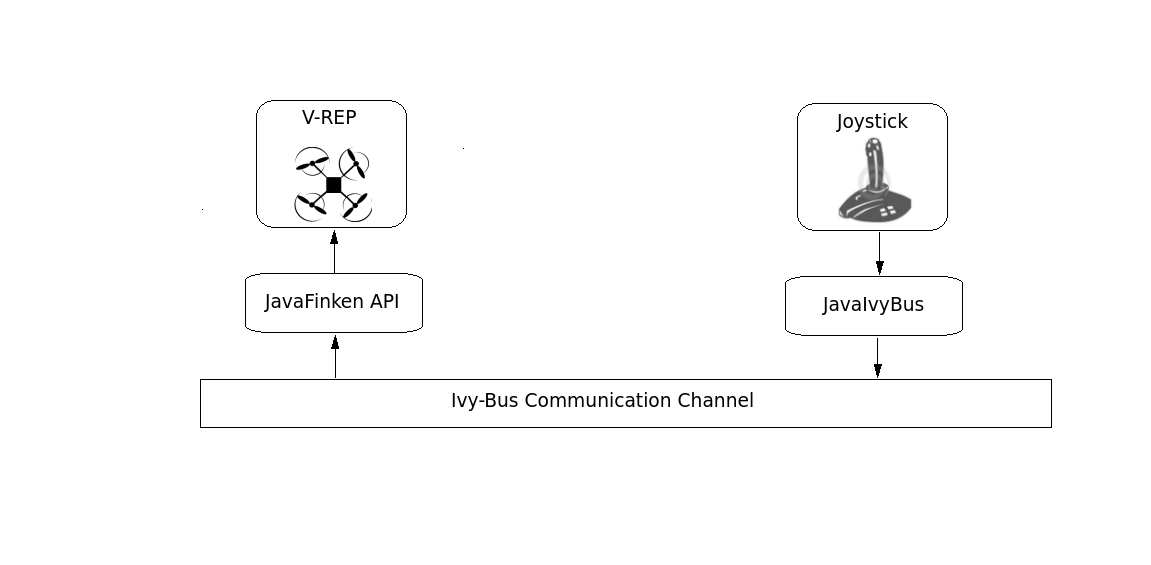
\includegraphics[scale=0.5]{FinkenHIL.png}
 \end{center}
  \caption{Finken Hardware-in-the-loop\label{fig:finkenHIL}}
\end{figure}

The HIL evaluation was implemented as a separate project - \textit{JavaFinkenSimHil}. 
It uses the Java external library \href{https://java.net/projects/jinput}{JInput} for reading the inputs from the joystick. 
The already created \textit{JavaIvyBus} module, which was discussed in \ref{sec:ivyBusImplementation}, is used to connect the Joystick to the Ivy-Bus. \\

The \textit{Joystick} class has as a local variable the class \textit{JoystickBusNode}, which extends the abstract \textit{AbsIvyBusNode}, thus being able to communicate on the common Ivy-Bus network. \\

The \textit{Joystick} class polls the data from the Joystick device at 50 Mhz and sends them to the \textit{JoystickBusNode}, which on the other hand encapsulates the data in a FINKEN\_ROTORCRAFT\_FP message and publishes it on the bus. \\ 

The FINKEN\_ROTORCRAFT\_FP is the message that the real Quadcopter uses to publish its pitch, yaw and roll angles. 
Since the Joystick fakes the real Quadcopter, the JavaFinkenApp receives the message as if coming from the real one, thus not even a single line of code had to be changed in the JavaFinkenApp, in order to use the HIL evaluation. \\

As a result of the evaluation we came to the following conclusions:

\begin{itemize}
\item{The controlling of the Quadcopter was very precise and accurate. 
We ware able to make any manoeuvre and flight path as desired. \\ 

When flying with the Joystick, one can get a real feeling of the Quadcopter flight dynamics and behaviour}.

\item{We experienced challenges with keeping the Quadcopter at a level height, using the throttle levers of the Joystick. 
It turned out, that keeping a level height was a matter of eye-hand coordination. \\

Even the slightest change to the thrust when hovering resulted in a strong accelaration in $z$-axis. 
Even if this behaviour corresponds to the real quadcopter, we identified it as a problem, as the hover thrust of the real quadcopter changes during flight time with the battery voltage. 
As a result, we decided to tune the throttle response of the virtual Quadcopter with a logistic curve as described in \ref{equ:logistic}}.

\end{itemize}

\section{Timing}
\subsection{VREP performance}
\begin{itemize}
\item{}
\item{}
\item{}
\item{}
\end{itemize}


\subsection{Timings in the Communication link}
\label{sec:commTiming}
\todo{communication delay}
\begin{itemize}
\item{}
\item{}
\item{mean delta t between sent messages, compare with the configured message frequency}
\item{possible buffering in AHRS}
\item{ run this with two or multiple quadrocopter}
\item{latency of JAVA link}
\end{itemize}


\todo{vrep simulation speed}
\todo{run vrep on the 10core computer in the lab, look at mean execution time}
\todo{add multiple copter}


\section{Accuracy}

To evaluate the accuracy of the simulation, we compared the orientation of the real FINken and the simulated model.  
We let the real FINken fly freely in the arena using the wall avoid control and linked the simulated FINken.
V-REP, paparazzi and the Java bridge were all run on the same machine.
The test flight which is referred to in the following was filmed.
The video, a screen recording of the simulation and the corresponding log files can be found online \todo{make raw data available} \todo{insert link to raw data}
The real quadcopter has some issues with the yaw angle. 
A cause for this is that the magnetometer does not provide reliable values indoors, due to interferences of electro-magnetic fields.
The sensors of the FINken are symmetrical, so yaw is not needed for regular movements.
Thus, it is tried to keep the copters orientation around the $z$ axis more or less stable.
The flight chose

The pitch and roll angles of the simulated FINken are more interesting.
When we logged the values via the telemetry link of paparazzi, and compared them to the values exported from the simulation, we noticed a time offset. 
This is not surprising, as we don't use an absolute reference time, but it made it impossible to directly compare the orientation logs.
To get a meaningful graphic, we manually resampled the logs and put them on a common time base.
Characteristic patterns were used to achieve a common time base.
In \ref{pic:pitchResponse} can be seen that the simulated FINken nicely adopts the real FINken's movements. 
The first spike at about $7s$ shows the takeoff. 
From $12s$ to $22s$ it can be seen how the real FINken got close to a wall and started to avoid it. 
The flight was stopped after about $43s$, the huge spikes at the end of the graph show how the response when the copter fell to the ground.
\begin{figure}
	\begin{center}
	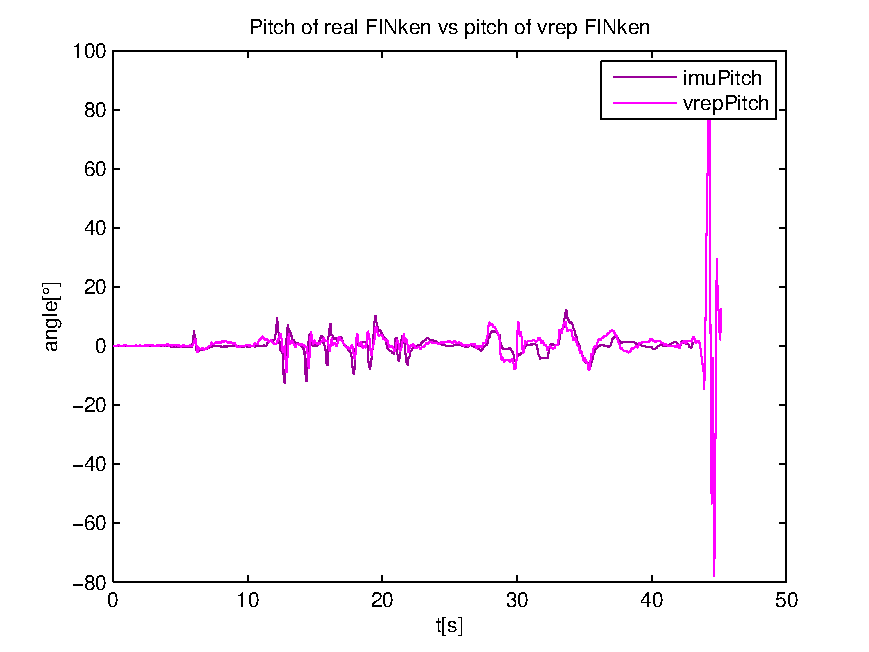
\includegraphics[width=\textwidth]{pitch}
	\caption{Pitch angles of simulated FINken and real FINken}
	\label{pic:pitchResponse}
	\end{center}
\end{figure}

A more detailed plot of the pitch comparison is shown in \ref{pic:pitchDetail}.
Every spike of the real FINkens movement is directly followed by a spike in the same direction of the simulated FINken.
The smaller movements do not correspond exactly, as the simulated copter contains its own attitude controller.
Thus, keeping the simulated FINken stable in air has a higher priority than following the real copter's movements.
The graph shows some points, e.g. before $17s$ where movement of the simulated FINken appears to precede the real FINken's movement.
This can have two possible explanations.
Firstly, as mentioned before, the time base was readjusted manually.
Thus, it might be possible, that as explained in \ref{sec:commTiming} \todo{write the explanation}, that the values were sent with a wrong timestamp that wasn't corrected during the adjustment, or even made worse by the resampling.
Secondly,  the controller of the simulated FINken's controller has the same goal as the real FINken, namely to keep the copter stable. 
In the following, it could be possible, that both controllers are going to apply the same changes and that the virtual one is slightly faster.
 

\begin{figure}
	\begin{center}
	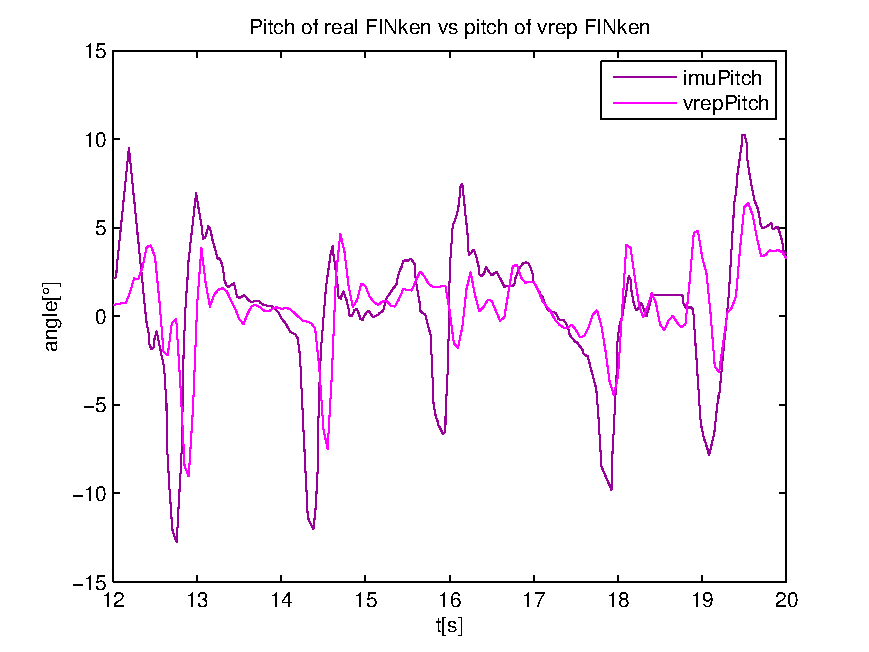
\includegraphics[width=\textwidth]{pitch_detail}
	\caption{Pitch angles of simulated FINken and real FINken}
	\label{pic:pitchDetail}
	\end{center}
\end{figure}

Interestingly, the roll of the FINkens as shown in \ref{fig:rollDetail} doesn't fit as well as the pitch, despite having identical controllers.
In this flight, we observed some logging error in V-REP. 
The huge

It can be seen, that the virtual FINken tries to follow the movements, but
\todo{add plot with roll spikes and pitch plot}
\begin{figure}
	\begin{center}
	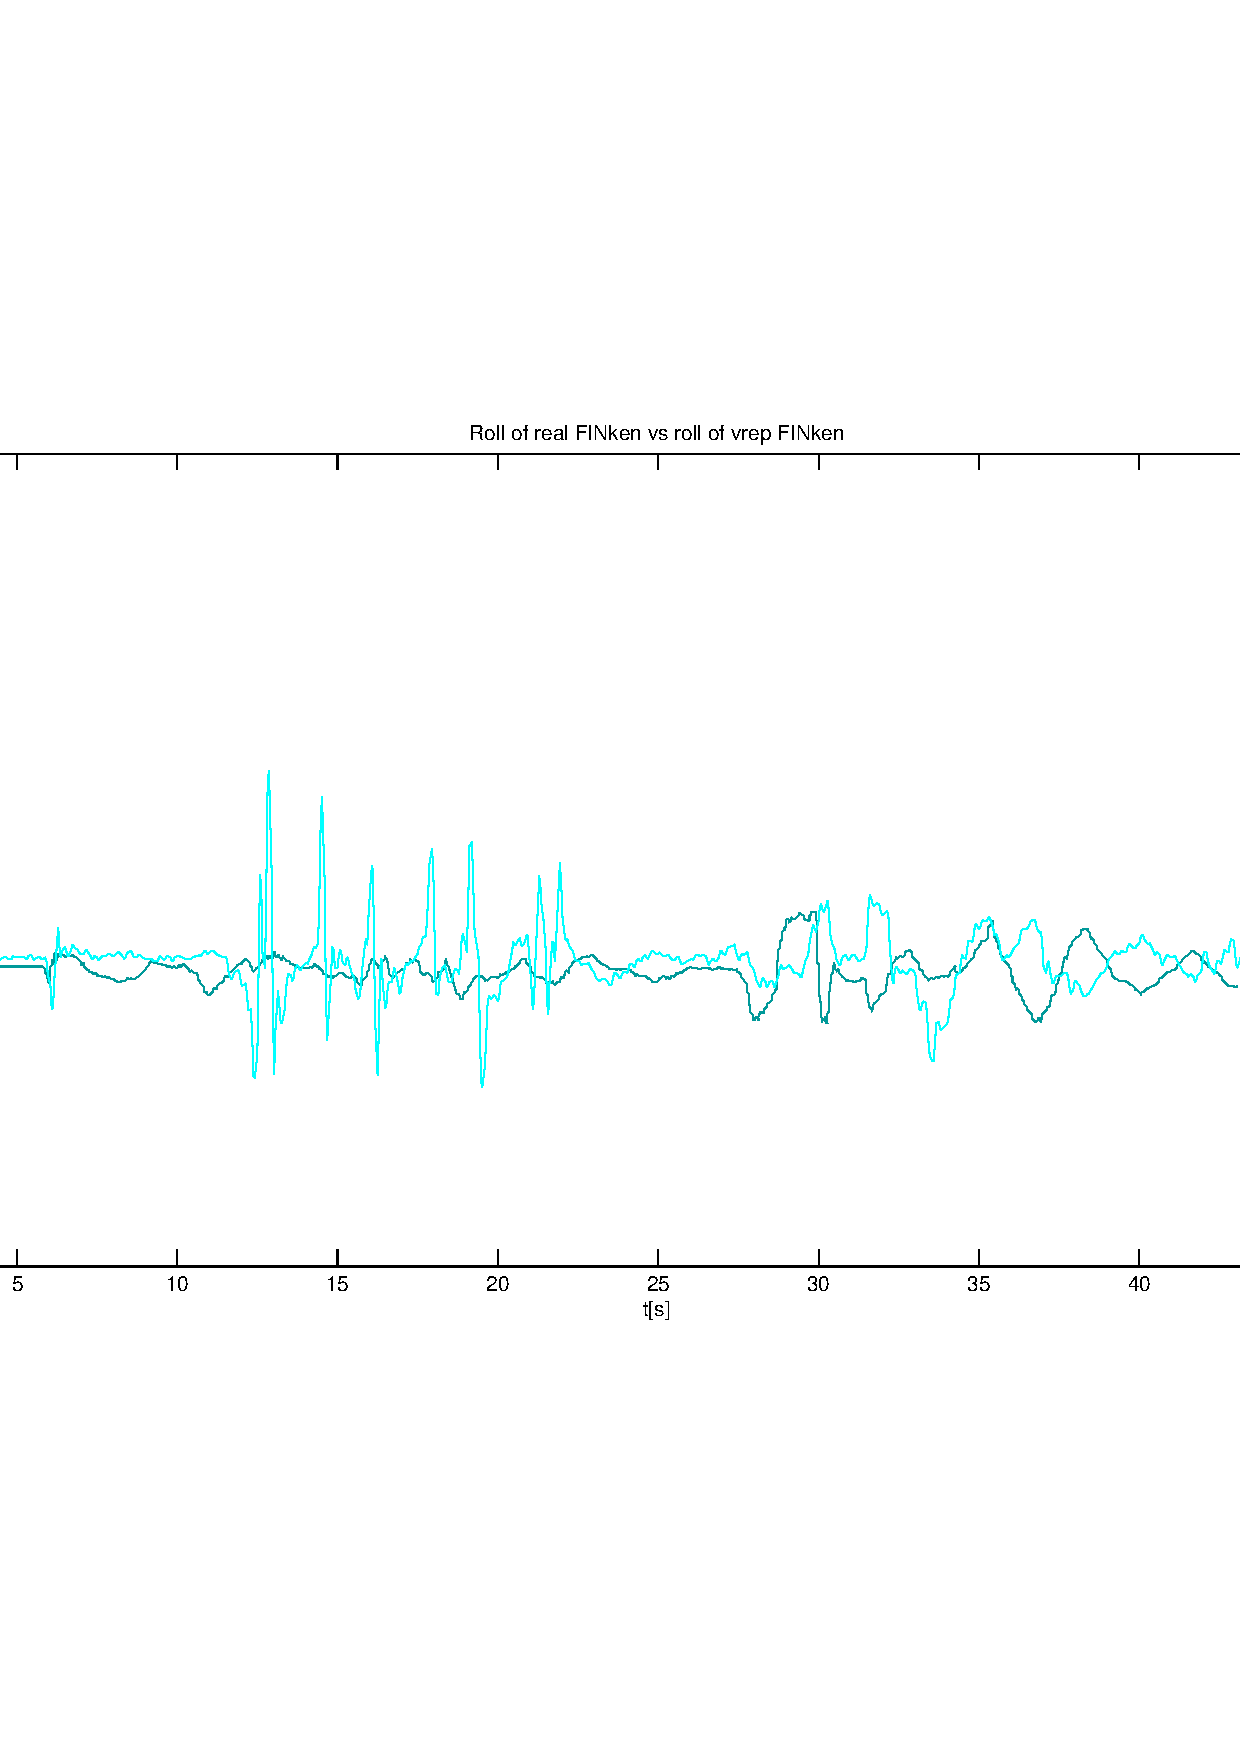
\includegraphics[width=\textwidth]{roll}
	\caption{Roll angles of simulated FINken and real FINken}
	\label{pic:rollResponse}
	\end{center}
\end{figure}


\todo{explanation for roll spikes: vreps internal handling of shapes; maybe copter and "IMU" are not moved at the same time? }
\todo{filter values? }
\begin{itemize}
\item{plot graph of euler angles}
\item{highlight start of drift, other interesting elements?}
\item{plot difference between graphs}

\end{itemize}


Eventually we wanted to evaluate to what extend the path of the flying quadrocopter matches the path of the simulated quadcopter. V-REP provides an easy way to plot the two dimensional position of the quadrocopter and draw the flying path, but our real quadrocopter does not have a positioning system and its position estimation is not possible.\\ In order to estimate the position we have used the MEDUSA localization system developed in our faculty [add reference to the paper]. The system calculates the two dimensional position of a mobile robot moving in a rectangular arena, using eight proximity sensors and a gyroscope. It uses the yaw angle of the robot and the distances to the walls from the proximity sensors to calculate a set of possible positions, where the quadrocopter could be. Then it moves through all possible points and calculates the distances, that the proximity sensors should read at that particular point and angle of rotation. Comparing the real readings from the quadrocopter proximity sensors and the calculated distances, a probability function is calculated, that indicates the probability that the real quadrocopter is situated at the particular point. The point with the highest probability is chosen for the quadcopter position.\\
The MEDUSA positioning system turned out to be an easy and fast way to get an estimation of the position, since our quadcopter has four ultrasound sensors, positioned at 90 degrees from each other, and a gyroscope, which provides the angle of rotation. The fact, that the original positioning system uses eight distance sensors was not disturbing, since it is possible to estimate the position even with two sensors. But a higher number of sensors provides more fault-tolerance to the system and more accuracy. It was also not necessary to implement the algorithm in the firmware of the quadcopter. We used the log file, that the Paparazzi software uses to write the sensor data and fetch the sensor readings from there using a Matlab script. Only a minor changes ware required in the configuration of the sensor numbers, the sensors maximum range and the size of the arena.\\
On \ref{fig:matlabPosEstimation} you can see the calculated possible positions and the quadcopter positioned at the point with the highest possibility value. The lines represent the ultrasound sensors and the length of the lines depict the maximum sensor range. The red fractions of the lines show the actual distance measured by the sensor. 

\begin{figure}[h!]
 \begin{center}
  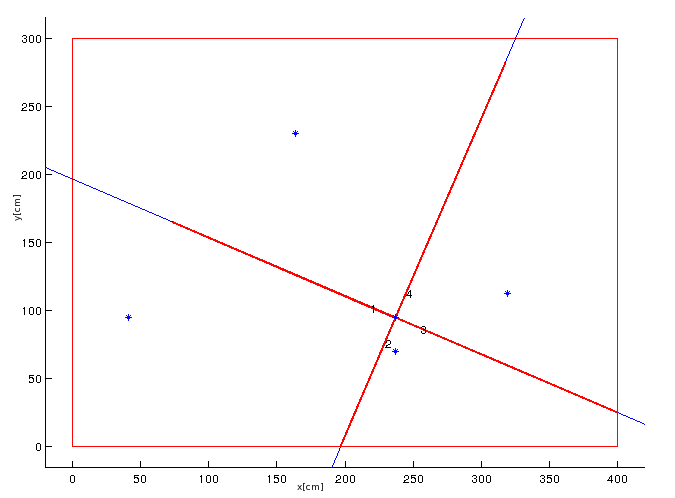
\includegraphics[scale=0.7]{MatlabPositionEstimation.png}
 \end{center}
  \caption{position estimation\label{fig:matlabPosEstimation}}
\end{figure}

The positioning system relies on accurate sensor readings to provide a precise position estimation. Our gyroscope provides noisy estimation of the yaw angle and the distance sensors are also quite noisy. Since our quadcopter is equipped with just four distance sensors, the localization system cannot tolerate the noise as good as with eight sensors. For this reasons an accurate position estimation could not be expected, but it should provide some reference estimation of the flying path. On \ref{fig:matlabPosPath} you can see the results of the position estimation. Each position has been marked with a blue star, so that we can see where the quadcopter has been. It is not possible to show the actual flying path as a function of time, but it shows which parts of the arena had been occupied by the quadcopter during the flight. \ref{fig:vrepPosPath} shows the flight path of the simulated quadcopter in the V-REP. As in \ref{fig:matlabPosPath} it does not shows the trajectory as a function of time, but just the occupied positions during the flight. The x and y axes of the plot show the V-REP scene arena and the small rectangle represents the flight arena.

\begin{figure}[h!]
 \begin{center}
  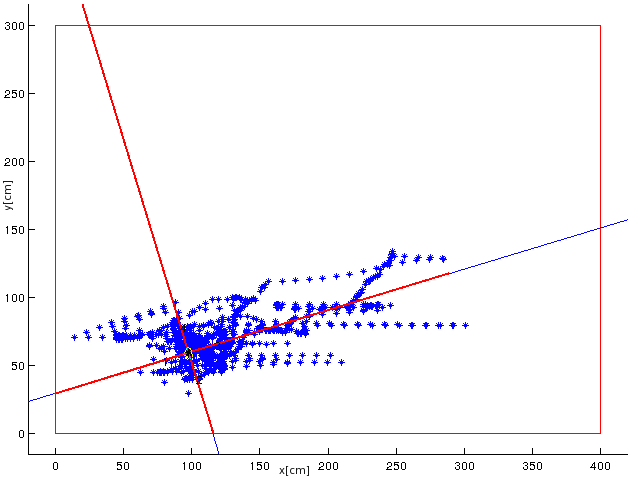
\includegraphics[scale=0.7]{MatlabPositionPath.png}
 \end{center}
  \caption{Estimated flight path\label{fig:matlabPosPath}}
\end{figure}

\begin{figure}[h!]
 \begin{center}
  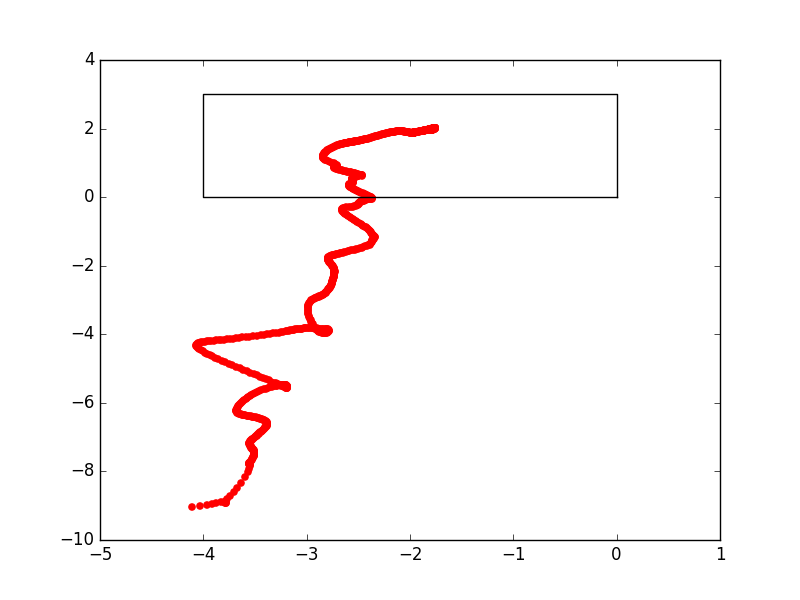
\includegraphics[scale=0.7]{vrepPath.png}
 \end{center}
  \caption{V-REP flight path\label{fig:vrepPosPath}}
\end{figure}

The estimated positions on \ref{fig:matlabPosPath} are very scattered, due to the fact that the localization system cannot estimate the position with a big accuracy. In the worst case, as a correct position was assumed one of the calculated possible points, which was far away from the previous estimated position. This creates a big jumps in the path, which does not coincide with the real flight path. The scattered plot and the jumps are caused by the noisy sensor measurements. A couple of attempts to filter the sensor readings ware made, but the plot still looked scattered to a significant extend. Also a Kalman Filter was implemented to eliminate the big jumps between the current and previous quadcopter positions, but the results ware still not satisfying.\\
On the other hand \ref{fig:vrepPosPath} shows a clear flying path, due to the fact that the position is not estimated, but taken directly from the V-REP environment. The graph shows how the quadcopter drifts and to what extend it flies away from the arena.\\
Eventually we came to the conclusion, that the used approach for position estimation was not good enough for our needs and a detailed comparison between the flying paths of the real and simulated quadcopter could not be done at this stage. However the working group has the intention to build a camera positioning system and track the quadcopter position with a camera mounted on the top of the arena.



\chapter{Conclusion}
\label{sec:conclusion}


\section{Reached goals}
\begin{itemize}
\item{a stable simulation was built}
\item{the simulation of multiple quadcopters is possible in near real time}
\item{a java program was build that can read and write on the ivy bus paparazzi uses}
\item{the java program can communicate with both VREP and paparazzi}
\item{orientation messages from the quadcopter can be sent to the simulation in less than a simulation time step}
\item{the virtual quadcopter resonds fast to command messages}
\item{
A Java API was build, that manages the V-REP scene and communication to the quadcopters. The API is very modular and comprises of several stand alone projects, each of which can be reused for other projects and mixed-reality simulations. The software architecture was build according to the SOLID principles and other design-patterns. The design uses abstraction layers between the modules, which make it possible 
}

\item{for a short time, until noise and possibly missing value induce a drift that can't be corrected with just internal measurements, it can be observed how the virtual copter follows the movements of a real one}
\end{itemize}




\section{Future Work}
\begin{itemize}
\item{enhance the stability of the mixed reality simulation}
\item{include the sensor data from the optical flow and ultrasound sensors for the positioning of the virtual quadcopter}
\item{implement real swarm algorithms with the framework}
\item{}
\end{itemize}
%Die Beurteilung ist einer der wichtigsten Abschnitte der Arbeit
%- Sie enthält die Quintessenz des gesamten Projektes
%Viele lesen nur die Einführung und die Beurteilung an
%- Hier muss also alles Wichtige drin stehen!
%Hier beweisen Sie dass Sie …
%- die Aufgabe und deren Bedeutung verstanden haben
%- die Ergebnisse richtig zu interpretieren vermögen
%- wissen, worauf es bei diese Arbeit ankam




% example for definition
%      \begin{definitionnonum} [Hierarchische Struktur] 
%      Wenn eine Softwarestruktur als Menge von Komponenten  und Relationen zwischen den Komponenten beschrieben wird, gilt diese Struktur als hierarchisch, wenn eine Relation oder ein Prädikat $R(\alpha, \beta)$ über Paaren dieser Komponenten Schichten folgendermaßen beschreiben kann: 
%      \begin{itemize} 
%      \item{Schicht 0 ist eine Menge von Komponenten $\alpha$, sodass  kein $\beta$ mit $R(\alpha,\beta)$ existiert} 
%      \item{Schicht $i$ ist eine Menge von Komponenten $\alpha$ ist, sodass auf Level $i-1$ ein $\beta$ existiert mit $R(\alpha,\beta)$ und alle $\gamma$ für $R(\alpha,\gamma)$ in der Schicht $i-1$ oder niedriger liegen} 
%      \end{itemize}
%      \end{definitionnonum}
      


% example for drawing      
%              \tikzstyle{decision} = [diamond, draw, fill=blue!20,
%    text width=4.5em, text badly centered, node distance=2.5cm, inner sep=0pt]
%\tikzstyle{block} = [rectangle, draw, fill=blue!20,
%    text width=5em, text centered, rounded corners, minimum height=4em]
%\tikzstyle{line} = [draw, very thick, color=black!50, -latex']
%\tikzstyle{cloud} = [draw, ellipse,fill=red!20, node distance=2.5cm,
%    minimum height=2em]
%\tikzstyle{node} = [draw, ellipse, node distance=2.5cm,
%    minimum height=2em]
%\tikzstyle{fullnode}= [draw, ellipse,fill=black!20, node distance=2.5cm,
%    minimum height =2em]
%\begin{figure}[h]
%\begin{center}
%\begin{tikzpicture}[scale=2, node distance = 2cm, auto]
%    % Place nodes
%  \node[node](b1){$b_1$};
%   \node[node, below of=b1, right of=b1](b3){$b_3$};
% \node[node, right of=b3, above of=b3](b2){$b_2$};
%
%
%\path [->, densely dotted] (b1) edge node{e} (b2);
%\path [->] (b1) edge (b3);
%\path [->] (b3) edge (b2);
%\path [->, dashed] (b1) edge[bend right] node[left]{$e_1$}(b3);
%\path [->,dashed] (b3) edge[bend right]  node[right]{$e_2$} (b2);
%\end{tikzpicture}
%\caption{Beispiel Gesetz von Demeter}
%\end{center}
%\end{figure}




% example for equation   
%\begin{equation}
%   L_{GvD}(a) = \sum_{b_i \in B(a)} L_{GvD}(b_i)
%\end{equation}
%    
      


%*********************************************************************%
% APPENDIX                                                            %
%*********************************************************************%

%\appendix
%\ifgerman{\chapter{Anhang}}{\chapter{Appendix}}
\label{appedixa}

\todots

%*********************************************************************%
% LITERATURE                                                          %
%*********************************************************************%

\cleardoublepage
\phantomsection
\addcontentsline{toc}{chapter}{\bibname} % 
\bibliographystyle{alphadin} % plain gerplain abbrvnat unsrtnat alphag alpha
% in a thesis you have space... use full names
%\bibliography{literature/finkenLiterature}
\bibliography{docear/_data/14FD099F8F985QT959J90Z53U5ZUFPVWENJ2/default_files/MixedRealityReport}
% in a paper, space is limited. use abreviations
%\bibliography{../literature/IEEEabrv,../literature/MYabrv,../literature/literature}

%*********************************************************************%
% ERKLÄRUNG                                                           %
%*********************************************************************%

%\ifnotdraft{
%	\cleardoublepage
%	\phantomsection
%	\printindex
%	\thispagestyle{empty}
\vspace*{38\baselineskip}
\hbox to \textwidth{\hrulefill}
\par
Hiermit erkl\"are ich, dass ich die vorliegende Arbeit selbst\"andig verfasst und
keine anderen als die angegebenen Quellen und Hilfsmittel verwendet habe.

Magdeburg, den 29. November, 2013

%%%%%%%%%%%%%%%%%%%%%%%%%%%%%%%%%%%%%%%%%%%%%%%%%%%%%%%%%%%%%%%%%%%%%%%%
%% Hinweis:
%%
%% Diese Erklärung wird von der Prüfungsordnung für Diplomarbeiten 
%% verlangt und ist zu unterschreiben. Für Studienarbeiten ist diese
%% Erklärung nicht zwingend notwendig, schadet aber auch nicht.
%%%%%%%%%%%%%%%%%%%%%%%%%%%%%%%%%%%%%%%%%%%%%%%%%%%%%%%%%%%%%%%%%%%%%%%%
\clearpage

%}

\end{document}
